\documentclass[letterpaper,11pt]{article}

\usepackage{geometry}
\usepackage{pslatex}
\usepackage{fancyhdr}
\usepackage{graphicx}
\usepackage{color}
\usepackage{tikz}
\usepackage{setspace}
\usepackage{amssymb}

\geometry{ margin = 1.0in }

\pagestyle{fancy}
\lhead{{\bf Lecture 39}}
\chead{{\bf CMPSC 465 Fall 2020}}
\rhead{{\bf Mingfu Shao}}

\setlength\parindent{0em}
\setlength\parskip{8pt}
%\setlength{\fboxsep}{6pt}

\usepackage{amsthm}
\newtheoremstyle{mytheorem}
  {\parskip} % Space above
  {0em} % Space below
  {} % Body font
  {} % Indent amount
  {\bfseries} % Theorem head font
  {.} % Punctuation after theorem head
  {.5em} % Space after theorem head
  {} % Theorem head spec (can be left empty, meaning `normal')

\theoremstyle{mytheorem}
\newtheorem{definition}{Definition}
\newtheorem{property}{Property}
\newtheorem{claim}{Claim}
\newtheorem{fact}{Fact}
\newtheorem{corollary}{Corollary}

% for algorithms
\newcommand{\aaa}[1]{\hspace{0.65cm}\parbox[t]{15.3cm}{#1}}
\newcommand{\aab}[1]{\hspace{1.15cm}\parbox[t]{15.0cm}{#1}}
\newcommand{\aac}[1]{\hspace{1.65cm}\parbox[t]{15.0cm}{#1}}
\newcommand{\aad}[1]{\hspace{2.15cm}\parbox[t]{15.0cm}{#1}}
\newcommand{\aae}[1]{\hspace{2.65cm}\parbox[t]{15.0cm}{#1}}
\newcommand{\aaf}[1]{\hspace{3.15cm}\parbox[t]{15.0cm}{#1}}
\newcommand{\aaA}[2]{\hspace{0.5cm} {\tikz[overlay] \draw (0.1, -0.1) -- (0.1, #1 * -1.5em + 0.6em);} \parbox[t]{15.0cm}{#2}}
\newcommand{\aaB}[2]{\hspace{1.0cm} {\tikz[overlay] \draw (0.1, -0.1) -- (0.1, #1 * -1.5em + 0.6em);} \parbox[t]{15.0cm}{#2}}
\newcommand{\aaC}[2]{\hspace{1.5cm} {\tikz[overlay] \draw (0.1, -0.1) -- (0.1, #1 * -1.5em + 0.6em);} \parbox[t]{15.0cm}{#2}}
\newcommand{\aaD}[2]{\hspace{2.0cm} {\tikz[overlay] \draw (0.1, -0.1) -- (0.1, #1 * -1.5em + 0.6em);} \parbox[t]{15.0cm}{#2}}
\newcommand{\aaE}[2]{\hspace{2.5cm} {\tikz[overlay] \draw (0.1, -0.1) -- (0.1, #1 * -1.5em + 0.6em);} \parbox[t]{15.0cm}{#2}}
\newcommand{\xxx}{\par\vspace{0.1cm}}

\begin{document}

\section*{Maximum-Matching and Minimum-Vertex Cover of Bipartite Graphs}

\subsection*{Maximum-Matching vs.\ Minimum-Vertex Cover on General Undirected Graphs}

Let $G = (V, E)$ be an undirected graph. A \emph{matching} $M \subset E$ 
is a subset of edges of $G$ that does not have common vertices.
A matching is also called an \emph{independent edge set}.
See Figure~\ref{fig:matching} for an example.
Given an undirected graph, the so-called \emph{maximum-matching problem}
seeks a matching $M$ of $G$ such that the number of edges in the matching, i.e., $|M|$, 
is maximized.

\begin{figure}[h]
\centering{

\tikzset{every picture/.style={line width=0.75pt}} %set default line width to 0.75pt        

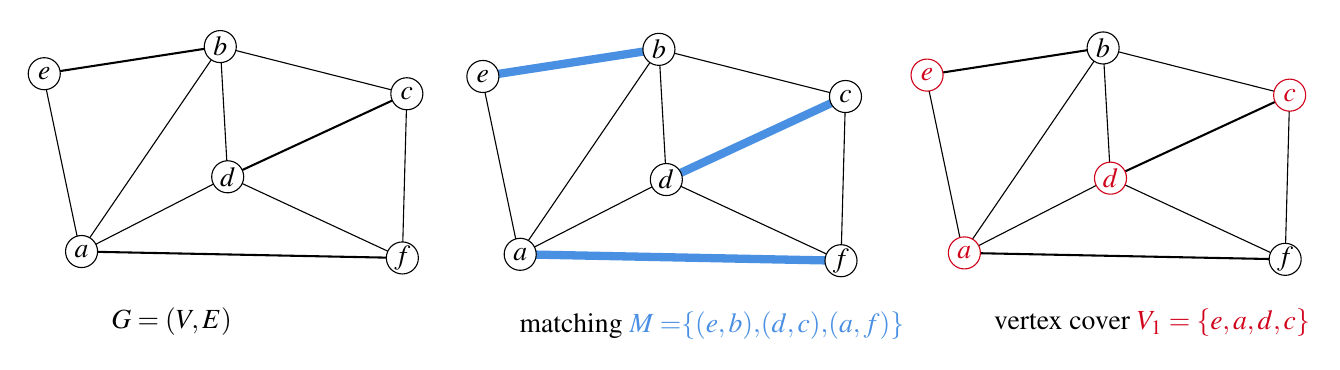
\begin{tikzpicture}[x=0.5pt,y=0.5pt,yscale=-1,xscale=1]
%uncomment if require: \path (0,237); %set diagram left start at 0, and has height of 237

%Straight Lines [id:da7485926733039977] 
\draw    (144.6,14.97) -- (43.43,163.09) ;
%Straight Lines [id:da4575120980127291] 
\draw [color={rgb, 255:red, 0; green, 0; blue, 0 }  ,draw opacity=1 ][line width=0.75]    (16.46,34.58) -- (143.69,14.97) ;
%Straight Lines [id:da9165715401778428] 
\draw    (16.46,34.58) -- (43.43,163.09) ;
%Straight Lines [id:da994182434786223] 
\draw [color={rgb, 255:red, 0; green, 0; blue, 0 }  ,draw opacity=1 ][line width=0.75]    (44.34,163.09) -- (276.17,167.73) ;
%Straight Lines [id:da9750224919648968] 
\draw    (149.95,109.07) -- (276.17,167.73) ;
%Straight Lines [id:da24348552449211425] 
\draw    (144.6,14.97) -- (149.95,109.07) ;
%Straight Lines [id:da16705340438790406] 
\draw    (144.6,14.97) -- (279.42,49.07) ;
%Straight Lines [id:da08663700279220432] 
\draw    (279.42,49.07) -- (276.17,167.73) ;
%Straight Lines [id:da16511775802360662] 
\draw [color={rgb, 255:red, 0; green, 0; blue, 0 }  ,draw opacity=1 ][line width=0.75]    (279.42,49.07) -- (149.95,109.07) ;
%Straight Lines [id:da4151454155794566] 
\draw    (149.95,109.07) -- (44.34,163.09) ;
%Shape: Ellipse [id:dp9133580928774087] 
\draw  [fill={rgb, 255:red, 255; green, 255; blue, 255 }  ,fill opacity=1 ] (5.79,34.58) .. controls (5.79,28.18) and (10.97,23) .. (17.37,23) .. controls (23.76,23) and (28.95,28.18) .. (28.95,34.58) .. controls (28.95,40.97) and (23.76,46.16) .. (17.37,46.16) .. controls (10.97,46.16) and (5.79,40.97) .. (5.79,34.58) -- cycle ;
%Shape: Ellipse [id:dp4005957609675306] 
\draw  [fill={rgb, 255:red, 255; green, 255; blue, 255 }  ,fill opacity=1 ] (133.02,14.97) .. controls (133.02,8.57) and (138.2,3.39) .. (144.6,3.39) .. controls (151,3.39) and (156.18,8.57) .. (156.18,14.97) .. controls (156.18,21.36) and (151,26.55) .. (144.6,26.55) .. controls (138.2,26.55) and (133.02,21.36) .. (133.02,14.97) -- cycle ;
%Shape: Ellipse [id:dp49214617921702164] 
\draw  [fill={rgb, 255:red, 255; green, 255; blue, 255 }  ,fill opacity=1 ] (267.84,49.07) .. controls (267.84,42.67) and (273.02,37.49) .. (279.42,37.49) .. controls (285.82,37.49) and (291,42.67) .. (291,49.07) .. controls (291,55.46) and (285.82,60.65) .. (279.42,60.65) .. controls (273.02,60.65) and (267.84,55.46) .. (267.84,49.07) -- cycle ;
%Shape: Ellipse [id:dp8440754424343925] 
\draw  [fill={rgb, 255:red, 255; green, 255; blue, 255 }  ,fill opacity=1 ] (138.37,109.07) .. controls (138.37,102.68) and (143.55,97.49) .. (149.95,97.49) .. controls (156.34,97.49) and (161.53,102.68) .. (161.53,109.07) .. controls (161.53,115.47) and (156.34,120.65) .. (149.95,120.65) .. controls (143.55,120.65) and (138.37,115.47) .. (138.37,109.07) -- cycle ;
%Shape: Ellipse [id:dp20660183368429152] 
\draw  [fill={rgb, 255:red, 255; green, 255; blue, 255 }  ,fill opacity=1 ] (32.76,163.09) .. controls (32.76,156.7) and (37.94,151.51) .. (44.34,151.51) .. controls (50.73,151.51) and (55.92,156.7) .. (55.92,163.09) .. controls (55.92,169.49) and (50.73,174.67) .. (44.34,174.67) .. controls (37.94,174.67) and (32.76,169.49) .. (32.76,163.09) -- cycle ;
%Shape: Ellipse [id:dp4098192910838151] 
\draw  [fill={rgb, 255:red, 255; green, 255; blue, 255 }  ,fill opacity=1 ] (264.59,167.73) .. controls (264.59,161.33) and (269.77,156.15) .. (276.17,156.15) .. controls (282.56,156.15) and (287.75,161.33) .. (287.75,167.73) .. controls (287.75,174.13) and (282.56,179.31) .. (276.17,179.31) .. controls (269.77,179.31) and (264.59,174.13) .. (264.59,167.73) -- cycle ;
%Straight Lines [id:da6233481480623783] 
\draw    (461.6,16.97) -- (360.43,165.09) ;
%Straight Lines [id:da9901942575404544] 
\draw [color={rgb, 255:red, 74; green, 144; blue, 226 }  ,draw opacity=1 ][line width=3]    (333.46,36.58) -- (460.69,16.97) ;
%Straight Lines [id:da3790939323014558] 
\draw    (333.46,36.58) -- (360.43,165.09) ;
%Straight Lines [id:da42115713644274366] 
\draw [color={rgb, 255:red, 74; green, 144; blue, 226 }  ,draw opacity=1 ][line width=3]    (361.34,165.09) -- (593.17,169.73) ;
%Straight Lines [id:da8702690824311631] 
\draw    (466.95,111.07) -- (593.17,169.73) ;
%Straight Lines [id:da34939805445985417] 
\draw    (461.6,16.97) -- (466.95,111.07) ;
%Straight Lines [id:da04544520748950576] 
\draw    (461.6,16.97) -- (596.42,51.07) ;
%Straight Lines [id:da5361594760285122] 
\draw    (596.42,51.07) -- (593.17,169.73) ;
%Straight Lines [id:da10465085418843478] 
\draw [color={rgb, 255:red, 74; green, 144; blue, 226 }  ,draw opacity=1 ][line width=3]    (596.42,51.07) -- (466.95,111.07) ;
%Straight Lines [id:da555393377892622] 
\draw    (466.95,111.07) -- (361.34,165.09) ;
%Shape: Ellipse [id:dp39324544068995604] 
\draw  [fill={rgb, 255:red, 255; green, 255; blue, 255 }  ,fill opacity=1 ] (322.79,36.58) .. controls (322.79,30.18) and (327.97,25) .. (334.37,25) .. controls (340.76,25) and (345.95,30.18) .. (345.95,36.58) .. controls (345.95,42.97) and (340.76,48.16) .. (334.37,48.16) .. controls (327.97,48.16) and (322.79,42.97) .. (322.79,36.58) -- cycle ;
%Shape: Ellipse [id:dp8663152391911655] 
\draw  [fill={rgb, 255:red, 255; green, 255; blue, 255 }  ,fill opacity=1 ] (450.02,16.97) .. controls (450.02,10.57) and (455.2,5.39) .. (461.6,5.39) .. controls (468,5.39) and (473.18,10.57) .. (473.18,16.97) .. controls (473.18,23.36) and (468,28.55) .. (461.6,28.55) .. controls (455.2,28.55) and (450.02,23.36) .. (450.02,16.97) -- cycle ;
%Shape: Ellipse [id:dp9564869279164044] 
\draw  [fill={rgb, 255:red, 255; green, 255; blue, 255 }  ,fill opacity=1 ] (584.84,51.07) .. controls (584.84,44.67) and (590.02,39.49) .. (596.42,39.49) .. controls (602.82,39.49) and (608,44.67) .. (608,51.07) .. controls (608,57.46) and (602.82,62.65) .. (596.42,62.65) .. controls (590.02,62.65) and (584.84,57.46) .. (584.84,51.07) -- cycle ;
%Shape: Ellipse [id:dp14244956479013948] 
\draw  [fill={rgb, 255:red, 255; green, 255; blue, 255 }  ,fill opacity=1 ] (455.37,111.07) .. controls (455.37,104.68) and (460.55,99.49) .. (466.95,99.49) .. controls (473.34,99.49) and (478.53,104.68) .. (478.53,111.07) .. controls (478.53,117.47) and (473.34,122.65) .. (466.95,122.65) .. controls (460.55,122.65) and (455.37,117.47) .. (455.37,111.07) -- cycle ;
%Shape: Ellipse [id:dp3916752397044988] 
\draw  [fill={rgb, 255:red, 255; green, 255; blue, 255 }  ,fill opacity=1 ] (349.76,165.09) .. controls (349.76,158.7) and (354.94,153.51) .. (361.34,153.51) .. controls (367.73,153.51) and (372.92,158.7) .. (372.92,165.09) .. controls (372.92,171.49) and (367.73,176.67) .. (361.34,176.67) .. controls (354.94,176.67) and (349.76,171.49) .. (349.76,165.09) -- cycle ;
%Shape: Ellipse [id:dp6775141746120102] 
\draw  [fill={rgb, 255:red, 255; green, 255; blue, 255 }  ,fill opacity=1 ] (581.59,169.73) .. controls (581.59,163.33) and (586.77,158.15) .. (593.17,158.15) .. controls (599.56,158.15) and (604.75,163.33) .. (604.75,169.73) .. controls (604.75,176.13) and (599.56,181.31) .. (593.17,181.31) .. controls (586.77,181.31) and (581.59,176.13) .. (581.59,169.73) -- cycle ;
%Straight Lines [id:da991028078692109] 
\draw    (782.6,15.97) -- (681.43,164.09) ;
%Straight Lines [id:da8020042074548936] 
\draw [color={rgb, 255:red, 0; green, 0; blue, 0 }  ,draw opacity=1 ][line width=0.75]    (654.46,35.58) -- (781.69,15.97) ;
%Straight Lines [id:da5410354625843318] 
\draw    (654.46,35.58) -- (681.43,164.09) ;
%Straight Lines [id:da1284005435452643] 
\draw [color={rgb, 255:red, 0; green, 0; blue, 0 }  ,draw opacity=1 ][line width=0.75]    (682.34,164.09) -- (914.17,168.73) ;
%Straight Lines [id:da4841445577516499] 
\draw    (787.95,110.07) -- (914.17,168.73) ;
%Straight Lines [id:da3189236797568633] 
\draw    (782.6,15.97) -- (787.95,110.07) ;
%Straight Lines [id:da24633327282247075] 
\draw    (782.6,15.97) -- (917.42,50.07) ;
%Straight Lines [id:da666695835406161] 
\draw    (917.42,50.07) -- (914.17,168.73) ;
%Straight Lines [id:da31804257401559455] 
\draw [color={rgb, 255:red, 0; green, 0; blue, 0 }  ,draw opacity=1 ][line width=0.75]    (917.42,50.07) -- (787.95,110.07) ;
%Straight Lines [id:da6699316806179542] 
\draw    (787.95,110.07) -- (682.34,164.09) ;
%Shape: Ellipse [id:dp818344887208882] 
\draw  [color={rgb, 255:red, 208; green, 2; blue, 27 }  ,draw opacity=1 ][fill={rgb, 255:red, 255; green, 255; blue, 255 }  ,fill opacity=1 ] (643.79,35.58) .. controls (643.79,29.18) and (648.97,24) .. (655.37,24) .. controls (661.76,24) and (666.95,29.18) .. (666.95,35.58) .. controls (666.95,41.97) and (661.76,47.16) .. (655.37,47.16) .. controls (648.97,47.16) and (643.79,41.97) .. (643.79,35.58) -- cycle ;
%Shape: Ellipse [id:dp5629283730413089] 
\draw  [fill={rgb, 255:red, 255; green, 255; blue, 255 }  ,fill opacity=1 ] (771.02,15.97) .. controls (771.02,9.57) and (776.2,4.39) .. (782.6,4.39) .. controls (789,4.39) and (794.18,9.57) .. (794.18,15.97) .. controls (794.18,22.36) and (789,27.55) .. (782.6,27.55) .. controls (776.2,27.55) and (771.02,22.36) .. (771.02,15.97) -- cycle ;
%Shape: Ellipse [id:dp21443256600205352] 
\draw  [color={rgb, 255:red, 208; green, 2; blue, 27 }  ,draw opacity=1 ][fill={rgb, 255:red, 255; green, 255; blue, 255 }  ,fill opacity=1 ] (905.84,50.07) .. controls (905.84,43.67) and (911.02,38.49) .. (917.42,38.49) .. controls (923.82,38.49) and (929,43.67) .. (929,50.07) .. controls (929,56.46) and (923.82,61.65) .. (917.42,61.65) .. controls (911.02,61.65) and (905.84,56.46) .. (905.84,50.07) -- cycle ;
%Shape: Ellipse [id:dp17023173827913307] 
\draw  [color={rgb, 255:red, 208; green, 2; blue, 27 }  ,draw opacity=1 ][fill={rgb, 255:red, 255; green, 255; blue, 255 }  ,fill opacity=1 ] (776.37,110.07) .. controls (776.37,103.68) and (781.55,98.49) .. (787.95,98.49) .. controls (794.34,98.49) and (799.53,103.68) .. (799.53,110.07) .. controls (799.53,116.47) and (794.34,121.65) .. (787.95,121.65) .. controls (781.55,121.65) and (776.37,116.47) .. (776.37,110.07) -- cycle ;
%Shape: Ellipse [id:dp21431691922786544] 
\draw  [color={rgb, 255:red, 208; green, 2; blue, 27 }  ,draw opacity=1 ][fill={rgb, 255:red, 255; green, 255; blue, 255 }  ,fill opacity=1 ] (670.76,164.09) .. controls (670.76,157.7) and (675.94,152.51) .. (682.34,152.51) .. controls (688.73,152.51) and (693.92,157.7) .. (693.92,164.09) .. controls (693.92,170.49) and (688.73,175.67) .. (682.34,175.67) .. controls (675.94,175.67) and (670.76,170.49) .. (670.76,164.09) -- cycle ;
%Shape: Ellipse [id:dp6777828112816564] 
\draw  [fill={rgb, 255:red, 255; green, 255; blue, 255 }  ,fill opacity=1 ] (902.59,168.73) .. controls (902.59,162.33) and (907.77,157.15) .. (914.17,157.15) .. controls (920.56,157.15) and (925.75,162.33) .. (925.75,168.73) .. controls (925.75,175.13) and (920.56,180.31) .. (914.17,180.31) .. controls (907.77,180.31) and (902.59,175.13) .. (902.59,168.73) -- cycle ;

% Text Node
\draw (17.37,34.58) node   [align=left] {$\displaystyle e$};
% Text Node
\draw (144.6,14.97) node   [align=left] {$\displaystyle b$};
% Text Node
\draw (279.42,49.07) node   [align=left] {$\displaystyle c$};
% Text Node
\draw (149.95,109.07) node   [align=left] {$\displaystyle d$};
% Text Node
\draw (44.34,163.09) node   [align=left] {$\displaystyle a$};
% Text Node
\draw (276.17,167.73) node   [align=left] {$\displaystyle f$};
% Text Node
\draw (64,202) node [anchor=north west][inner sep=0.75pt]   [align=left] {$\displaystyle G=( V,E)$};
% Text Node
\draw (334.37,36.58) node   [align=left] {$\displaystyle e$};
% Text Node
\draw (461.6,16.97) node   [align=left] {$\displaystyle b$};
% Text Node
\draw (596.42,51.07) node   [align=left] {$\displaystyle c$};
% Text Node
\draw (466.95,111.07) node   [align=left] {$\displaystyle d$};
% Text Node
\draw (361.34,165.09) node   [align=left] {$\displaystyle a$};
% Text Node
\draw (593.17,169.73) node   [align=left] {$\displaystyle f$};
% Text Node
\draw (359,205) node [anchor=north west][inner sep=0.75pt]   [align=left] {matching $\displaystyle \textcolor[rgb]{0.29,0.56,0.89}{M=}\textcolor[rgb]{0.29,0.56,0.89}{\{}\textcolor[rgb]{0.29,0.56,0.89}{(}\textcolor[rgb]{0.29,0.56,0.89}{e,b}\textcolor[rgb]{0.29,0.56,0.89}{)}\textcolor[rgb]{0.29,0.56,0.89}{,}\textcolor[rgb]{0.29,0.56,0.89}{(}\textcolor[rgb]{0.29,0.56,0.89}{d,c}\textcolor[rgb]{0.29,0.56,0.89}{)}\textcolor[rgb]{0.29,0.56,0.89}{,}\textcolor[rgb]{0.29,0.56,0.89}{(}\textcolor[rgb]{0.29,0.56,0.89}{a,f}\textcolor[rgb]{0.29,0.56,0.89}{)}\textcolor[rgb]{0.29,0.56,0.89}{\}}$};
% Text Node
\draw (655.37,35.58) node  [color={rgb, 255:red, 208; green, 2; blue, 27 }  ,opacity=1 ] [align=left] {$\displaystyle e$};
% Text Node
\draw (782.6,15.97) node   [align=left] {$\displaystyle b$};
% Text Node
\draw (917.42,50.07) node  [color={rgb, 255:red, 208; green, 2; blue, 27 }  ,opacity=1 ] [align=left] {$\displaystyle c$};
% Text Node
\draw (787.95,110.07) node  [color={rgb, 255:red, 208; green, 2; blue, 27 }  ,opacity=1 ] [align=left] {$\displaystyle d$};
% Text Node
\draw (682.34,164.09) node  [color={rgb, 255:red, 208; green, 2; blue, 27 }  ,opacity=1 ] [align=left] {$\displaystyle a$};
% Text Node
\draw (914.17,168.73) node   [align=left] {$\displaystyle f$};
% Text Node
\draw (702,203) node [anchor=north west][inner sep=0.75pt]   [align=left] {vertex cover $\displaystyle \textcolor[rgb]{0.82,0.01,0.11}{V_{1} =\{e,a,d,c\}}$};


\end{tikzpicture}

}
\caption{A matching $M$ and a vertex cover $V_1$ of an undirected graph $G$. 
Note that $M$ is also a \emph{maximum matching} of $G$ and $V_1$ is also a minimum vertex cover of $G$.}
\label{fig:matching}
\end{figure}

Recall that a \emph{vertex cover} of an undirected graph $G = (V, E)$ is defined
as a subset of vertices $V_1\subset V$ that \emph{covers} all edges~(see Lecture~34 and Lecture~35).
There exists a connection between matchings and vertex covers of an undirected graph, stated below.

\begin{claim}
Let $G = (V, E)$ be an undirected graph. Let $M$ be any matching of $G$ and let $V_1$ be any vertex cover of $G$.
Then we have $|M| \le |V_1|$.
\end{claim}

\emph{Proof.} Since $V_1$ is a vertex cover, it covers all edges of $G$, in particular, all edges of $M$.
Since $M$ is a matching, all edges in $M$ don't share vertices, so it requires $|M|$ vertices to cover edges in $M$.
%as each edge in $M$ needs a new vertex to cover it.  
Combined, we have $|M| \le |V_1|$. \qed

So, the size of any vertex cover is an upper bound of the size of any matching. We again can virsualize
such relationship with Figure~\ref{fig:meet}. Clearly, if we can find a matching $M$ and a vertex cover $V_1$
(of the same undirected graph $G$) satisfying that $|M| = |V_1|$, then $M$ must be a maximum matching 
and $V_1$ must be a minimum vertex cover.

\begin{figure}[h]
\centering{

\tikzset{every picture/.style={line width=0.75pt}} %set default line width to 0.75pt        

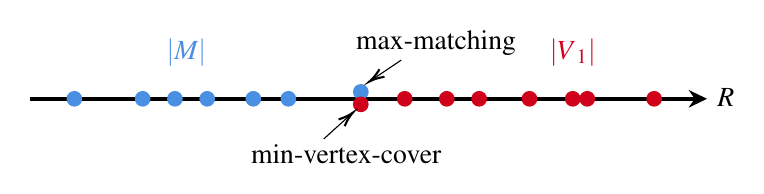
\begin{tikzpicture}[x=0.5pt,y=0.5pt,yscale=-1,xscale=1]
%uncomment if require: \path (0,126); %set diagram left start at 0, and has height of 126

%Straight Lines [id:da6845720994983642] 
\draw [line width=1.5]    (7,59) -- (492.5,59) ;
\draw [shift={(496.5,59)}, rotate = 180] [fill={rgb, 255:red, 0; green, 0; blue, 0 }  ][line width=0.08]  [draw opacity=0] (13.4,-6.43) -- (0,0) -- (13.4,6.44) -- (8.9,0) -- cycle    ;
%Shape: Circle [id:dp5839925944461984] 
\draw  [color={rgb, 255:red, 74; green, 144; blue, 226 }  ,draw opacity=1 ][fill={rgb, 255:red, 74; green, 144; blue, 226 }  ,fill opacity=1 ] (241,54) .. controls (241,51.1) and (243.35,48.75) .. (246.25,48.75) .. controls (249.15,48.75) and (251.5,51.1) .. (251.5,54) .. controls (251.5,56.9) and (249.15,59.25) .. (246.25,59.25) .. controls (243.35,59.25) and (241,56.9) .. (241,54) -- cycle ;
%Shape: Circle [id:dp34886579289539754] 
\draw  [color={rgb, 255:red, 74; green, 144; blue, 226 }  ,draw opacity=1 ][fill={rgb, 255:red, 74; green, 144; blue, 226 }  ,fill opacity=1 ] (188.65,59) .. controls (188.65,56.1) and (191,53.75) .. (193.9,53.75) .. controls (196.8,53.75) and (199.15,56.1) .. (199.15,59) .. controls (199.15,61.9) and (196.8,64.25) .. (193.9,64.25) .. controls (191,64.25) and (188.65,61.9) .. (188.65,59) -- cycle ;
%Shape: Circle [id:dp4135235202894928] 
\draw  [color={rgb, 255:red, 74; green, 144; blue, 226 }  ,draw opacity=1 ][fill={rgb, 255:red, 74; green, 144; blue, 226 }  ,fill opacity=1 ] (34,59) .. controls (34,56.1) and (36.35,53.75) .. (39.25,53.75) .. controls (42.15,53.75) and (44.5,56.1) .. (44.5,59) .. controls (44.5,61.9) and (42.15,64.25) .. (39.25,64.25) .. controls (36.35,64.25) and (34,61.9) .. (34,59) -- cycle ;
%Shape: Circle [id:dp20365687038540725] 
\draw  [color={rgb, 255:red, 74; green, 144; blue, 226 }  ,draw opacity=1 ][fill={rgb, 255:red, 74; green, 144; blue, 226 }  ,fill opacity=1 ] (83.33,59) .. controls (83.33,56.1) and (85.68,53.75) .. (88.58,53.75) .. controls (91.48,53.75) and (93.83,56.1) .. (93.83,59) .. controls (93.83,61.9) and (91.48,64.25) .. (88.58,64.25) .. controls (85.68,64.25) and (83.33,61.9) .. (83.33,59) -- cycle ;
%Shape: Circle [id:dp001936474221955753] 
\draw  [color={rgb, 255:red, 74; green, 144; blue, 226 }  ,draw opacity=1 ][fill={rgb, 255:red, 74; green, 144; blue, 226 }  ,fill opacity=1 ] (106.66,59) .. controls (106.66,56.1) and (109.01,53.75) .. (111.91,53.75) .. controls (114.81,53.75) and (117.16,56.1) .. (117.16,59) .. controls (117.16,61.9) and (114.81,64.25) .. (111.91,64.25) .. controls (109.01,64.25) and (106.66,61.9) .. (106.66,59) -- cycle ;
%Shape: Circle [id:dp8083671983789567] 
\draw  [color={rgb, 255:red, 74; green, 144; blue, 226 }  ,draw opacity=1 ][fill={rgb, 255:red, 74; green, 144; blue, 226 }  ,fill opacity=1 ] (129.99,59) .. controls (129.99,56.1) and (132.34,53.75) .. (135.24,53.75) .. controls (138.14,53.75) and (140.49,56.1) .. (140.49,59) .. controls (140.49,61.9) and (138.14,64.25) .. (135.24,64.25) .. controls (132.34,64.25) and (129.99,61.9) .. (129.99,59) -- cycle ;
%Shape: Circle [id:dp9076802577362922] 
\draw  [color={rgb, 255:red, 74; green, 144; blue, 226 }  ,draw opacity=1 ][fill={rgb, 255:red, 74; green, 144; blue, 226 }  ,fill opacity=1 ] (163.32,59) .. controls (163.32,56.1) and (165.67,53.75) .. (168.57,53.75) .. controls (171.47,53.75) and (173.82,56.1) .. (173.82,59) .. controls (173.82,61.9) and (171.47,64.25) .. (168.57,64.25) .. controls (165.67,64.25) and (163.32,61.9) .. (163.32,59) -- cycle ;
%Shape: Circle [id:dp4236178447115101] 
\draw  [color={rgb, 255:red, 208; green, 2; blue, 27 }  ,draw opacity=1 ][fill={rgb, 255:red, 208; green, 2; blue, 27 }  ,fill opacity=1 ] (241,63) .. controls (241,60.1) and (243.35,57.75) .. (246.25,57.75) .. controls (249.15,57.75) and (251.5,60.1) .. (251.5,63) .. controls (251.5,65.9) and (249.15,68.25) .. (246.25,68.25) .. controls (243.35,68.25) and (241,65.9) .. (241,63) -- cycle ;
%Shape: Circle [id:dp5050758022328539] 
\draw  [color={rgb, 255:red, 208; green, 2; blue, 27 }  ,draw opacity=1 ][fill={rgb, 255:red, 208; green, 2; blue, 27 }  ,fill opacity=1 ] (272.76,59) .. controls (272.76,56.1) and (275.11,53.75) .. (278.01,53.75) .. controls (280.91,53.75) and (283.26,56.1) .. (283.26,59) .. controls (283.26,61.9) and (280.91,64.25) .. (278.01,64.25) .. controls (275.11,64.25) and (272.76,61.9) .. (272.76,59) -- cycle ;
%Shape: Circle [id:dp8576227272464049] 
\draw  [color={rgb, 255:red, 208; green, 2; blue, 27 }  ,draw opacity=1 ][fill={rgb, 255:red, 208; green, 2; blue, 27 }  ,fill opacity=1 ] (303.14,59) .. controls (303.14,56.1) and (305.49,53.75) .. (308.39,53.75) .. controls (311.29,53.75) and (313.64,56.1) .. (313.64,59) .. controls (313.64,61.9) and (311.29,64.25) .. (308.39,64.25) .. controls (305.49,64.25) and (303.14,61.9) .. (303.14,59) -- cycle ;
%Shape: Circle [id:dp40578843932984965] 
\draw  [color={rgb, 255:red, 208; green, 2; blue, 27 }  ,draw opacity=1 ][fill={rgb, 255:red, 208; green, 2; blue, 27 }  ,fill opacity=1 ] (326.52,59) .. controls (326.52,56.1) and (328.87,53.75) .. (331.77,53.75) .. controls (334.67,53.75) and (337.02,56.1) .. (337.02,59) .. controls (337.02,61.9) and (334.67,64.25) .. (331.77,64.25) .. controls (328.87,64.25) and (326.52,61.9) .. (326.52,59) -- cycle ;
%Shape: Circle [id:dp2060326184335437] 
\draw  [color={rgb, 255:red, 208; green, 2; blue, 27 }  ,draw opacity=1 ][fill={rgb, 255:red, 208; green, 2; blue, 27 }  ,fill opacity=1 ] (362.9,59) .. controls (362.9,56.1) and (365.25,53.75) .. (368.15,53.75) .. controls (371.05,53.75) and (373.4,56.1) .. (373.4,59) .. controls (373.4,61.9) and (371.05,64.25) .. (368.15,64.25) .. controls (365.25,64.25) and (362.9,61.9) .. (362.9,59) -- cycle ;
%Shape: Circle [id:dp7156703955132185] 
\draw  [color={rgb, 255:red, 208; green, 2; blue, 27 }  ,draw opacity=1 ][fill={rgb, 255:red, 208; green, 2; blue, 27 }  ,fill opacity=1 ] (394.16,59) .. controls (394.16,56.1) and (396.51,53.75) .. (399.41,53.75) .. controls (402.31,53.75) and (404.66,56.1) .. (404.66,59) .. controls (404.66,61.9) and (402.31,64.25) .. (399.41,64.25) .. controls (396.51,64.25) and (394.16,61.9) .. (394.16,59) -- cycle ;
%Shape: Circle [id:dp5714468634699819] 
\draw  [color={rgb, 255:red, 208; green, 2; blue, 27 }  ,draw opacity=1 ][fill={rgb, 255:red, 208; green, 2; blue, 27 }  ,fill opacity=1 ] (404.66,59) .. controls (404.66,56.1) and (407.01,53.75) .. (409.91,53.75) .. controls (412.81,53.75) and (415.16,56.1) .. (415.16,59) .. controls (415.16,61.9) and (412.81,64.25) .. (409.91,64.25) .. controls (407.01,64.25) and (404.66,61.9) .. (404.66,59) -- cycle ;
%Shape: Circle [id:dp338221725625915] 
\draw  [color={rgb, 255:red, 208; green, 2; blue, 27 }  ,draw opacity=1 ][fill={rgb, 255:red, 208; green, 2; blue, 27 }  ,fill opacity=1 ] (453,59) .. controls (453,56.1) and (455.35,53.75) .. (458.25,53.75) .. controls (461.15,53.75) and (463.5,56.1) .. (463.5,59) .. controls (463.5,61.9) and (461.15,64.25) .. (458.25,64.25) .. controls (455.35,64.25) and (453,61.9) .. (453,59) -- cycle ;
%Straight Lines [id:da046923477941067104] 
\draw    (219.5,88) -- (239.02,70.34) ;
\draw [shift={(240.5,69)}, rotate = 497.86] [color={rgb, 255:red, 0; green, 0; blue, 0 }  ][line width=0.75]    (10.93,-3.29) .. controls (6.95,-1.4) and (3.31,-0.3) .. (0,0) .. controls (3.31,0.3) and (6.95,1.4) .. (10.93,3.29)   ;
%Straight Lines [id:da008869050799750533] 
\draw    (275.5,31) -- (254.16,45.38) ;
\draw [shift={(252.5,46.5)}, rotate = 326.02] [color={rgb, 255:red, 0; green, 0; blue, 0 }  ][line width=0.75]    (10.93,-3.29) .. controls (6.95,-1.4) and (3.31,-0.3) .. (0,0) .. controls (3.31,0.3) and (6.95,1.4) .. (10.93,3.29)   ;

% Text Node
\draw (502,50) node [anchor=north west][inner sep=0.75pt]   [align=left] {$\displaystyle R$};
% Text Node
\draw (104,14) node [anchor=north west][inner sep=0.75pt]   [align=left] {$\displaystyle \textcolor[rgb]{0.29,0.56,0.89}{|M|}$};
% Text Node
\draw (381,14) node [anchor=north west][inner sep=0.75pt]   [align=left] {$\displaystyle \textcolor[rgb]{0.82,0.01,0.11}{|V}\textcolor[rgb]{0.82,0.01,0.11}{_{1}}\textcolor[rgb]{0.82,0.01,0.11}{|}$};
% Text Node
\draw (165,90) node [anchor=north west][inner sep=0.75pt]   [align=left] {min-vertex-cover};
% Text Node
\draw (241,8) node [anchor=north west][inner sep=0.75pt]   [align=left] {max-matching};


\end{tikzpicture}

}
\caption{Each blue point represents the size of a matching and each red point represents the size of a vertex cover,
of the same undirected graph. Do they always meet?}
\label{fig:meet}
\end{figure}

Does for \emph{every} undirected graph there always exists a matching $M$ and a 
vertex cover $V_1$ that satisfies $|M| = |V_1|$?
The answer is no, and Figure~\ref{fig:matching} gives such an example.
A more informative example is a triangle: a graph $G = (V, E)$ with $V = \{a,b,c\}$ and $E = \{(a,b), (b,c), (c,a)\}$.
In a triangle, the maximum matching includes one edge, but to cover all 3 edges we need 2 vertices.
In fact, an undirected graph consists of an \emph{odd-length} cycle with $2m+1$ edges admits
a maximum matching with $m$ edges and a minimum vertex cover with $m+1$ vertices.
It seems that it's the odd-length cycles that results in a gap.
In fact, this is true. Following we will show that, if an undirected
graph $G$ does not contain odd-length cycle, then the size of its maximum matching
must be equal to the size of its minimum vertex cover. The proof is again constructive:
we will design an algorithm to find both, and show that they have equal size.


\subsection*{Maximum Matching of Bipartite Graphs}

We first give an equivalent~(and nice) characterization of an undirected graph without odd-length cycles.
\begin{fact}
An undirected graph $G$ does not contain odd-length cycle if and only if $G$ is a \emph{bipartite} graph.
\end{fact}

An \emph{bipartite} graph, usually written as $G = (X\cup Y, E)$, is an undirected graph
whose vertices can be separated into two disjoint subsets $X$ and $Y$ such that all its edges
must span $X$ and $Y$~(i.e., every edge $e = (u,v)\in E$ must satisfy $u\in X$ and $v\in Y$).
See Figure~\ref{fig:bipartite}.
Clearly, any cycle in a bipartite graph~(for example, the cycle $(b,h,c,f)$ in Figure~\ref{fig:bipartite})
must be of even-length, as it need to visit $X$ and $Y$ alternately.
(We skip the proof of the other side of this fact.)

\begin{figure}[h]
\centering{

\tikzset{every picture/.style={line width=0.75pt}} %set default line width to 0.75pt        

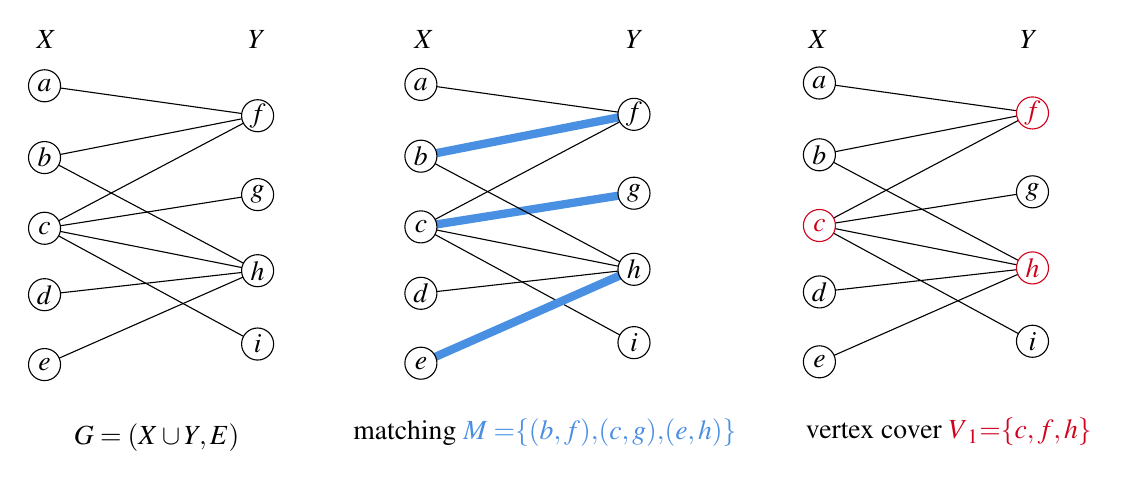
\begin{tikzpicture}[x=0.5pt,y=0.5pt,yscale=-1,xscale=1]
%uncomment if require: \path (0,316); %set diagram left start at 0, and has height of 316

%Straight Lines [id:da6233481480623783] 
\draw    (173.67,69.73) -- (19.68,99.97) ;
%Straight Lines [id:da3790939323014558] 
\draw    (19.68,48.09) -- (173.67,69.73) ;
%Straight Lines [id:da555393377892622] 
\draw    (173.67,69.73) -- (19.68,151.07) ;
%Straight Lines [id:da17109149534540602] 
\draw    (173.67,181.73) -- (19.68,151.07) ;
%Straight Lines [id:da8491552224613422] 
\draw    (173.67,234.73) -- (19.68,151.07) ;
%Straight Lines [id:da6111412207445381] 
\draw    (173.67,126.73) -- (19.68,151.07) ;
%Straight Lines [id:da40246334963984653] 
\draw    (173.67,181.73) -- (19.68,199.07) ;
%Straight Lines [id:da8951096474536266] 
\draw    (173.67,181.73) -- (19.68,249.58) ;
%Straight Lines [id:da442507224234595] 
\draw    (173.67,181.73) -- (19.68,99.97) ;
%Shape: Ellipse [id:dp9133580928774087] 
\draw  [fill={rgb, 255:red, 255; green, 255; blue, 255 }  ,fill opacity=1 ] (8.1,249.58) .. controls (8.1,243.18) and (13.29,238) .. (19.68,238) .. controls (26.08,238) and (31.26,243.18) .. (31.26,249.58) .. controls (31.26,255.97) and (26.08,261.16) .. (19.68,261.16) .. controls (13.29,261.16) and (8.1,255.97) .. (8.1,249.58) -- cycle ;
%Shape: Ellipse [id:dp4005957609675306] 
\draw  [fill={rgb, 255:red, 255; green, 255; blue, 255 }  ,fill opacity=1 ] (8.1,99.97) .. controls (8.1,93.57) and (13.29,88.39) .. (19.68,88.39) .. controls (26.08,88.39) and (31.26,93.57) .. (31.26,99.97) .. controls (31.26,106.36) and (26.08,111.55) .. (19.68,111.55) .. controls (13.29,111.55) and (8.1,106.36) .. (8.1,99.97) -- cycle ;
%Shape: Ellipse [id:dp49214617921702164] 
\draw  [fill={rgb, 255:red, 255; green, 255; blue, 255 }  ,fill opacity=1 ] (8.1,151.07) .. controls (8.1,144.67) and (13.29,139.49) .. (19.68,139.49) .. controls (26.08,139.49) and (31.26,144.67) .. (31.26,151.07) .. controls (31.26,157.46) and (26.08,162.65) .. (19.68,162.65) .. controls (13.29,162.65) and (8.1,157.46) .. (8.1,151.07) -- cycle ;
%Shape: Ellipse [id:dp8440754424343925] 
\draw  [fill={rgb, 255:red, 255; green, 255; blue, 255 }  ,fill opacity=1 ] (8.1,199.07) .. controls (8.1,192.68) and (13.29,187.49) .. (19.68,187.49) .. controls (26.08,187.49) and (31.26,192.68) .. (31.26,199.07) .. controls (31.26,205.47) and (26.08,210.65) .. (19.68,210.65) .. controls (13.29,210.65) and (8.1,205.47) .. (8.1,199.07) -- cycle ;
%Shape: Ellipse [id:dp20660183368429152] 
\draw  [fill={rgb, 255:red, 255; green, 255; blue, 255 }  ,fill opacity=1 ] (8.1,48.09) .. controls (8.1,41.7) and (13.29,36.51) .. (19.68,36.51) .. controls (26.08,36.51) and (31.26,41.7) .. (31.26,48.09) .. controls (31.26,54.49) and (26.08,59.67) .. (19.68,59.67) .. controls (13.29,59.67) and (8.1,54.49) .. (8.1,48.09) -- cycle ;
%Shape: Ellipse [id:dp4098192910838151] 
\draw  [fill={rgb, 255:red, 255; green, 255; blue, 255 }  ,fill opacity=1 ] (162.09,69.73) .. controls (162.09,63.33) and (167.27,58.15) .. (173.67,58.15) .. controls (180.06,58.15) and (185.25,63.33) .. (185.25,69.73) .. controls (185.25,76.13) and (180.06,81.31) .. (173.67,81.31) .. controls (167.27,81.31) and (162.09,76.13) .. (162.09,69.73) -- cycle ;
%Shape: Ellipse [id:dp04818959761719954] 
\draw  [fill={rgb, 255:red, 255; green, 255; blue, 255 }  ,fill opacity=1 ] (162.09,126.73) .. controls (162.09,120.33) and (167.27,115.15) .. (173.67,115.15) .. controls (180.06,115.15) and (185.25,120.33) .. (185.25,126.73) .. controls (185.25,133.13) and (180.06,138.31) .. (173.67,138.31) .. controls (167.27,138.31) and (162.09,133.13) .. (162.09,126.73) -- cycle ;
%Shape: Ellipse [id:dp776083183452069] 
\draw  [fill={rgb, 255:red, 255; green, 255; blue, 255 }  ,fill opacity=1 ] (162.09,181.73) .. controls (162.09,175.33) and (167.27,170.15) .. (173.67,170.15) .. controls (180.06,170.15) and (185.25,175.33) .. (185.25,181.73) .. controls (185.25,188.13) and (180.06,193.31) .. (173.67,193.31) .. controls (167.27,193.31) and (162.09,188.13) .. (162.09,181.73) -- cycle ;
%Shape: Ellipse [id:dp943943166831801] 
\draw  [fill={rgb, 255:red, 255; green, 255; blue, 255 }  ,fill opacity=1 ] (162.09,234.73) .. controls (162.09,228.33) and (167.27,223.15) .. (173.67,223.15) .. controls (180.06,223.15) and (185.25,228.33) .. (185.25,234.73) .. controls (185.25,241.13) and (180.06,246.31) .. (173.67,246.31) .. controls (167.27,246.31) and (162.09,241.13) .. (162.09,234.73) -- cycle ;
%Straight Lines [id:da5762269873281055] 
\draw [color={rgb, 255:red, 74; green, 144; blue, 226 }  ,draw opacity=1 ][line width=3]    (445.67,68.73) -- (291.68,98.97) ;
%Straight Lines [id:da6557704374413869] 
\draw    (291.68,47.09) -- (445.67,68.73) ;
%Straight Lines [id:da37940197486810245] 
\draw    (445.67,68.73) -- (291.68,150.07) ;
%Straight Lines [id:da2489426088203095] 
\draw    (445.67,180.73) -- (291.68,150.07) ;
%Straight Lines [id:da614864797412136] 
\draw    (445.67,233.73) -- (291.68,150.07) ;
%Straight Lines [id:da19212175099205075] 
\draw [color={rgb, 255:red, 74; green, 144; blue, 226 }  ,draw opacity=1 ][line width=3]    (445.67,125.73) -- (291.68,150.07) ;
%Straight Lines [id:da318853764666447] 
\draw    (445.67,180.73) -- (291.68,198.07) ;
%Straight Lines [id:da3703675549768074] 
\draw [color={rgb, 255:red, 74; green, 144; blue, 226 }  ,draw opacity=1 ][line width=3]    (445.67,180.73) -- (291.68,248.58) ;
%Straight Lines [id:da8823098712187499] 
\draw    (445.67,180.73) -- (291.68,98.97) ;
%Shape: Ellipse [id:dp3095150063265397] 
\draw  [fill={rgb, 255:red, 255; green, 255; blue, 255 }  ,fill opacity=1 ] (280.1,248.58) .. controls (280.1,242.18) and (285.29,237) .. (291.68,237) .. controls (298.08,237) and (303.26,242.18) .. (303.26,248.58) .. controls (303.26,254.97) and (298.08,260.16) .. (291.68,260.16) .. controls (285.29,260.16) and (280.1,254.97) .. (280.1,248.58) -- cycle ;
%Shape: Ellipse [id:dp20721463292670939] 
\draw  [fill={rgb, 255:red, 255; green, 255; blue, 255 }  ,fill opacity=1 ] (280.1,98.97) .. controls (280.1,92.57) and (285.29,87.39) .. (291.68,87.39) .. controls (298.08,87.39) and (303.26,92.57) .. (303.26,98.97) .. controls (303.26,105.36) and (298.08,110.55) .. (291.68,110.55) .. controls (285.29,110.55) and (280.1,105.36) .. (280.1,98.97) -- cycle ;
%Shape: Ellipse [id:dp5446258401720914] 
\draw  [fill={rgb, 255:red, 255; green, 255; blue, 255 }  ,fill opacity=1 ] (280.1,150.07) .. controls (280.1,143.67) and (285.29,138.49) .. (291.68,138.49) .. controls (298.08,138.49) and (303.26,143.67) .. (303.26,150.07) .. controls (303.26,156.46) and (298.08,161.65) .. (291.68,161.65) .. controls (285.29,161.65) and (280.1,156.46) .. (280.1,150.07) -- cycle ;
%Shape: Ellipse [id:dp012444989815690533] 
\draw  [fill={rgb, 255:red, 255; green, 255; blue, 255 }  ,fill opacity=1 ] (280.1,198.07) .. controls (280.1,191.68) and (285.29,186.49) .. (291.68,186.49) .. controls (298.08,186.49) and (303.26,191.68) .. (303.26,198.07) .. controls (303.26,204.47) and (298.08,209.65) .. (291.68,209.65) .. controls (285.29,209.65) and (280.1,204.47) .. (280.1,198.07) -- cycle ;
%Shape: Ellipse [id:dp5639306398005206] 
\draw  [fill={rgb, 255:red, 255; green, 255; blue, 255 }  ,fill opacity=1 ] (280.1,47.09) .. controls (280.1,40.7) and (285.29,35.51) .. (291.68,35.51) .. controls (298.08,35.51) and (303.26,40.7) .. (303.26,47.09) .. controls (303.26,53.49) and (298.08,58.67) .. (291.68,58.67) .. controls (285.29,58.67) and (280.1,53.49) .. (280.1,47.09) -- cycle ;
%Shape: Ellipse [id:dp3692499940189833] 
\draw  [fill={rgb, 255:red, 255; green, 255; blue, 255 }  ,fill opacity=1 ] (434.09,68.73) .. controls (434.09,62.33) and (439.27,57.15) .. (445.67,57.15) .. controls (452.06,57.15) and (457.25,62.33) .. (457.25,68.73) .. controls (457.25,75.13) and (452.06,80.31) .. (445.67,80.31) .. controls (439.27,80.31) and (434.09,75.13) .. (434.09,68.73) -- cycle ;
%Shape: Ellipse [id:dp17469367724521878] 
\draw  [fill={rgb, 255:red, 255; green, 255; blue, 255 }  ,fill opacity=1 ] (434.09,125.73) .. controls (434.09,119.33) and (439.27,114.15) .. (445.67,114.15) .. controls (452.06,114.15) and (457.25,119.33) .. (457.25,125.73) .. controls (457.25,132.13) and (452.06,137.31) .. (445.67,137.31) .. controls (439.27,137.31) and (434.09,132.13) .. (434.09,125.73) -- cycle ;
%Shape: Ellipse [id:dp35472333728828986] 
\draw  [fill={rgb, 255:red, 255; green, 255; blue, 255 }  ,fill opacity=1 ] (434.09,180.73) .. controls (434.09,174.33) and (439.27,169.15) .. (445.67,169.15) .. controls (452.06,169.15) and (457.25,174.33) .. (457.25,180.73) .. controls (457.25,187.13) and (452.06,192.31) .. (445.67,192.31) .. controls (439.27,192.31) and (434.09,187.13) .. (434.09,180.73) -- cycle ;
%Shape: Ellipse [id:dp4084404782784946] 
\draw  [fill={rgb, 255:red, 255; green, 255; blue, 255 }  ,fill opacity=1 ] (434.09,233.73) .. controls (434.09,227.33) and (439.27,222.15) .. (445.67,222.15) .. controls (452.06,222.15) and (457.25,227.33) .. (457.25,233.73) .. controls (457.25,240.13) and (452.06,245.31) .. (445.67,245.31) .. controls (439.27,245.31) and (434.09,240.13) .. (434.09,233.73) -- cycle ;
%Straight Lines [id:da2461791334712684] 
\draw    (733.67,67.73) -- (579.68,97.97) ;
%Straight Lines [id:da45747325160291075] 
\draw    (579.68,46.09) -- (733.67,67.73) ;
%Straight Lines [id:da9670994187206017] 
\draw    (733.67,67.73) -- (579.68,149.07) ;
%Straight Lines [id:da75134152117505] 
\draw    (733.67,179.73) -- (579.68,149.07) ;
%Straight Lines [id:da3699894396868808] 
\draw    (733.67,232.73) -- (579.68,149.07) ;
%Straight Lines [id:da13352692532928045] 
\draw    (733.67,124.73) -- (579.68,149.07) ;
%Straight Lines [id:da12851059505065643] 
\draw    (733.67,179.73) -- (579.68,197.07) ;
%Straight Lines [id:da9630672080240875] 
\draw    (733.67,179.73) -- (579.68,247.58) ;
%Straight Lines [id:da43029644611033324] 
\draw    (733.67,179.73) -- (579.68,97.97) ;
%Shape: Ellipse [id:dp8625040314784665] 
\draw  [fill={rgb, 255:red, 255; green, 255; blue, 255 }  ,fill opacity=1 ] (568.1,247.58) .. controls (568.1,241.18) and (573.29,236) .. (579.68,236) .. controls (586.08,236) and (591.26,241.18) .. (591.26,247.58) .. controls (591.26,253.97) and (586.08,259.16) .. (579.68,259.16) .. controls (573.29,259.16) and (568.1,253.97) .. (568.1,247.58) -- cycle ;
%Shape: Ellipse [id:dp658489289612401] 
\draw  [fill={rgb, 255:red, 255; green, 255; blue, 255 }  ,fill opacity=1 ] (568.1,97.97) .. controls (568.1,91.57) and (573.29,86.39) .. (579.68,86.39) .. controls (586.08,86.39) and (591.26,91.57) .. (591.26,97.97) .. controls (591.26,104.36) and (586.08,109.55) .. (579.68,109.55) .. controls (573.29,109.55) and (568.1,104.36) .. (568.1,97.97) -- cycle ;
%Shape: Ellipse [id:dp6017085286802247] 
\draw  [color={rgb, 255:red, 208; green, 2; blue, 27 }  ,draw opacity=1 ][fill={rgb, 255:red, 255; green, 255; blue, 255 }  ,fill opacity=1 ] (568.1,149.07) .. controls (568.1,142.67) and (573.29,137.49) .. (579.68,137.49) .. controls (586.08,137.49) and (591.26,142.67) .. (591.26,149.07) .. controls (591.26,155.46) and (586.08,160.65) .. (579.68,160.65) .. controls (573.29,160.65) and (568.1,155.46) .. (568.1,149.07) -- cycle ;
%Shape: Ellipse [id:dp4350947131056553] 
\draw  [fill={rgb, 255:red, 255; green, 255; blue, 255 }  ,fill opacity=1 ] (568.1,197.07) .. controls (568.1,190.68) and (573.29,185.49) .. (579.68,185.49) .. controls (586.08,185.49) and (591.26,190.68) .. (591.26,197.07) .. controls (591.26,203.47) and (586.08,208.65) .. (579.68,208.65) .. controls (573.29,208.65) and (568.1,203.47) .. (568.1,197.07) -- cycle ;
%Shape: Ellipse [id:dp8450977689112541] 
\draw  [fill={rgb, 255:red, 255; green, 255; blue, 255 }  ,fill opacity=1 ] (568.1,46.09) .. controls (568.1,39.7) and (573.29,34.51) .. (579.68,34.51) .. controls (586.08,34.51) and (591.26,39.7) .. (591.26,46.09) .. controls (591.26,52.49) and (586.08,57.67) .. (579.68,57.67) .. controls (573.29,57.67) and (568.1,52.49) .. (568.1,46.09) -- cycle ;
%Shape: Ellipse [id:dp40264635353475564] 
\draw  [color={rgb, 255:red, 208; green, 2; blue, 27 }  ,draw opacity=1 ][fill={rgb, 255:red, 255; green, 255; blue, 255 }  ,fill opacity=1 ] (722.09,67.73) .. controls (722.09,61.33) and (727.27,56.15) .. (733.67,56.15) .. controls (740.06,56.15) and (745.25,61.33) .. (745.25,67.73) .. controls (745.25,74.13) and (740.06,79.31) .. (733.67,79.31) .. controls (727.27,79.31) and (722.09,74.13) .. (722.09,67.73) -- cycle ;
%Shape: Ellipse [id:dp532306356301902] 
\draw  [fill={rgb, 255:red, 255; green, 255; blue, 255 }  ,fill opacity=1 ] (722.09,124.73) .. controls (722.09,118.33) and (727.27,113.15) .. (733.67,113.15) .. controls (740.06,113.15) and (745.25,118.33) .. (745.25,124.73) .. controls (745.25,131.13) and (740.06,136.31) .. (733.67,136.31) .. controls (727.27,136.31) and (722.09,131.13) .. (722.09,124.73) -- cycle ;
%Shape: Ellipse [id:dp495488673758371] 
\draw  [color={rgb, 255:red, 208; green, 2; blue, 27 }  ,draw opacity=1 ][fill={rgb, 255:red, 255; green, 255; blue, 255 }  ,fill opacity=1 ] (722.09,179.73) .. controls (722.09,173.33) and (727.27,168.15) .. (733.67,168.15) .. controls (740.06,168.15) and (745.25,173.33) .. (745.25,179.73) .. controls (745.25,186.13) and (740.06,191.31) .. (733.67,191.31) .. controls (727.27,191.31) and (722.09,186.13) .. (722.09,179.73) -- cycle ;
%Shape: Ellipse [id:dp6018453398031668] 
\draw  [fill={rgb, 255:red, 255; green, 255; blue, 255 }  ,fill opacity=1 ] (722.09,232.73) .. controls (722.09,226.33) and (727.27,221.15) .. (733.67,221.15) .. controls (740.06,221.15) and (745.25,226.33) .. (745.25,232.73) .. controls (745.25,239.13) and (740.06,244.31) .. (733.67,244.31) .. controls (727.27,244.31) and (722.09,239.13) .. (722.09,232.73) -- cycle ;

% Text Node
\draw (19.68,249.58) node   [align=left] {$\displaystyle e$};
% Text Node
\draw (19.68,99.97) node   [align=left] {$\displaystyle b$};
% Text Node
\draw (19.68,151.07) node   [align=left] {$\displaystyle c$};
% Text Node
\draw (19.68,199.07) node   [align=left] {$\displaystyle d$};
% Text Node
\draw (19.68,48.09) node   [align=left] {$\displaystyle a$};
% Text Node
\draw (173.67,69.73) node   [align=left] {$\displaystyle f$};
% Text Node
\draw (39,290.5) node [anchor=north west][inner sep=0.75pt]   [align=left] {$\displaystyle G=( X\cup Y,E)$};
% Text Node
\draw (241,286.5) node [anchor=north west][inner sep=0.75pt]   [align=left] {matching $\displaystyle \textcolor[rgb]{0.29,0.56,0.89}{M=}\textcolor[rgb]{0.29,0.56,0.89}{\{}\textcolor[rgb]{0.29,0.56,0.89}{(}\textcolor[rgb]{0.29,0.56,0.89}{b,f}\textcolor[rgb]{0.29,0.56,0.89}{)}\textcolor[rgb]{0.29,0.56,0.89}{,}\textcolor[rgb]{0.29,0.56,0.89}{(}\textcolor[rgb]{0.29,0.56,0.89}{c,g}\textcolor[rgb]{0.29,0.56,0.89}{)}\textcolor[rgb]{0.29,0.56,0.89}{,}\textcolor[rgb]{0.29,0.56,0.89}{(}\textcolor[rgb]{0.29,0.56,0.89}{e,h}\textcolor[rgb]{0.29,0.56,0.89}{)}\textcolor[rgb]{0.29,0.56,0.89}{\}}$};
% Text Node
\draw (568,286.5) node [anchor=north west][inner sep=0.75pt]   [align=left] {vertex cover $\displaystyle \textcolor[rgb]{0.82,0.01,0.11}{V}\textcolor[rgb]{0.82,0.01,0.11}{_{1}}\textcolor[rgb]{0.82,0.01,0.11}{=}\textcolor[rgb]{0.82,0.01,0.11}{\{}\textcolor[rgb]{0.82,0.01,0.11}{c,f,h}\textcolor[rgb]{0.82,0.01,0.11}{\}}$};
% Text Node
\draw (173.67,126.73) node   [align=left] {$\displaystyle g$};
% Text Node
\draw (173.67,181.73) node   [align=left] {$\displaystyle h$};
% Text Node
\draw (173.67,234.73) node   [align=left] {$\displaystyle i$};
% Text Node
\draw (291.68,248.58) node   [align=left] {$\displaystyle e$};
% Text Node
\draw (291.68,98.97) node   [align=left] {$\displaystyle b$};
% Text Node
\draw (291.68,150.07) node   [align=left] {$\displaystyle c$};
% Text Node
\draw (291.68,198.07) node   [align=left] {$\displaystyle d$};
% Text Node
\draw (291.68,47.09) node   [align=left] {$\displaystyle a$};
% Text Node
\draw (445.67,68.73) node   [align=left] {$\displaystyle f$};
% Text Node
\draw (445.67,125.73) node   [align=left] {$\displaystyle g$};
% Text Node
\draw (445.67,180.73) node   [align=left] {$\displaystyle h$};
% Text Node
\draw (445.67,233.73) node   [align=left] {$\displaystyle i$};
% Text Node
\draw (579.68,247.58) node   [align=left] {$\displaystyle e$};
% Text Node
\draw (579.68,97.97) node   [align=left] {$\displaystyle b$};
% Text Node
\draw (579.68,149.07) node  [color={rgb, 255:red, 208; green, 2; blue, 27 }  ,opacity=1 ] [align=left] {$\displaystyle c$};
% Text Node
\draw (579.68,197.07) node   [align=left] {$\displaystyle d$};
% Text Node
\draw (579.68,46.09) node   [align=left] {$\displaystyle a$};
% Text Node
\draw (733.67,67.73) node  [color={rgb, 255:red, 208; green, 2; blue, 27 }  ,opacity=1 ] [align=left] {$\displaystyle f$};
% Text Node
\draw (733.67,124.73) node   [align=left] {$\displaystyle g$};
% Text Node
\draw (733.67,179.73) node  [color={rgb, 255:red, 208; green, 2; blue, 27 }  ,opacity=1 ] [align=left] {$\displaystyle h$};
% Text Node
\draw (733.67,232.73) node   [align=left] {$\displaystyle i$};
% Text Node
\draw (12,6.5) node [anchor=north west][inner sep=0.75pt]   [align=left] {$\displaystyle X$};
% Text Node
\draw (165,6.5) node [anchor=north west][inner sep=0.75pt]   [align=left] {$\displaystyle Y$};
% Text Node
\draw (285,6.5) node [anchor=north west][inner sep=0.75pt]   [align=left] {$\displaystyle X$};
% Text Node
\draw (438,6.5) node [anchor=north west][inner sep=0.75pt]   [align=left] {$\displaystyle Y$};
% Text Node
\draw (570,6.5) node [anchor=north west][inner sep=0.75pt]   [align=left] {$\displaystyle X$};
% Text Node
\draw (723,6.5) node [anchor=north west][inner sep=0.75pt]   [align=left] {$\displaystyle Y$};


\end{tikzpicture}

}
\caption{A bipartite graph $G = (X\cup Y, E)$, 
a maximum matching $M$, and a minimum vertex cover $V_1$ of $G$.  }
\label{fig:bipartite}
\end{figure}

We now design an algorithm to find one maximum matching $M$ of a given bipartite graph $G = (X\cup Y, E)$.
This algorithm will also give a vertex cover $V_1$ of $G$, and we will prove $|M| = |V_1|$.
This will therefore proves that $M$ is a maximum matching, $V_1$ is a minimum vertex cover, and that
for every bipartite graph the size of its maximum matching and minimum vertex cover are equal.

We will not design new algorithm for this bipartite maximum matching problem, although this has
been a classical problem in computer science and many algorithms exist~(check wikipedia).
To solve it, we will \emph{transform this problem into a maximum-flow problem}.
This typically consists of three steps:
\vspace*{-\topsep}
\begin{enumerate}
\item construct an instance of the maximum-flow problem, i.e., a network, based on the given instance, i.e., a bipartite graph;
\item solve the maximum-flow instance constructed in step 1~(using any existing algorithm);
\item construct the maximum matching of the given bipartite graph based on the optimal solution~(i.e., the maximum flow
of the constructed network) obtained in step~2.
\end{enumerate}

Step 2 can be done simply by calling an existing solver. Steps 1 and 3 are closely related.
How to construct the instance is another ``art'' part of algorithm design: usually it requires
trying and observing.

Here is a working approach. Given a bipartite graph $G = (X\cup Y, E)$, we construct
a network $G' = (V', E')$ with source $s$ sink $t$ and edge capacities $c$ as follows.
See Figure~\ref{fig:transform}.
We construct $G'$ by modifying $G$: not a surprise, the given bipartite graph is the main
body of $G'$.
We first add two new vertices, a source $s$ and a sink $t$, a step that is usually required
in transforming a problem into a maximum-flow problem.
That is, $V' = X\cup Y\cup \{s, t\}$.
Second, we add a new directed edge $(s,x)$ that connects the source to every vertex $x\in X$, 
and add a new directed edge $(y,t)$ that connects every vertex $y\in Y$ to the sink $t$. 
For every edge $(x,y)\in E$ with $x\in X$ and $y\in Y$ in the bipartite graph,
we then copy it to $G'$ and assign it with a direction pointing from $x$ to $y$.
Last, we set the capacity as 1 for every edge in $G'$, i.e., $c(e) = 1$ for every $e\in E'$.

\begin{figure}[h]
\centering{

\tikzset{every picture/.style={line width=0.75pt}} %set default line width to 0.75pt        

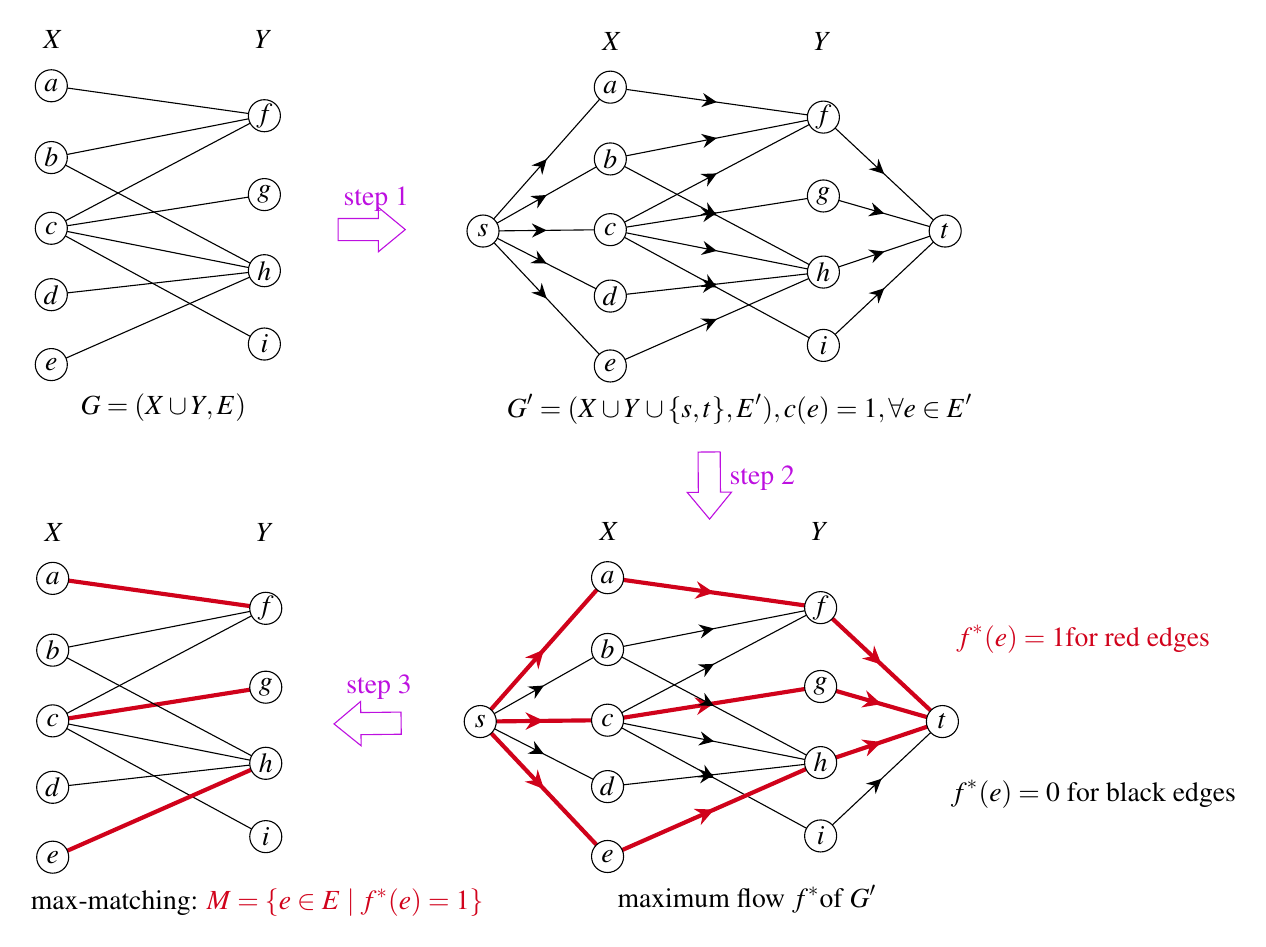
\begin{tikzpicture}[x=0.5pt,y=0.5pt,yscale=-1,xscale=1]
%uncomment if require: \path (0,664); %set diagram left start at 0, and has height of 664

%Straight Lines [id:da9104884328106918] 
\draw    (423.68,49.09) -- (331.68,153.07) ;
\draw [shift={(377.68,101.08)}, rotate = 131.5] [fill={rgb, 255:red, 0; green, 0; blue, 0 }  ][line width=0.08]  [draw opacity=0] (10.72,-5.15) -- (0,0) -- (10.72,5.15) -- (7.12,0) -- cycle    ;
%Straight Lines [id:da7681874141811359] 
\draw    (423.68,100.97) -- (331.68,153.07) ;
\draw [shift={(377.68,127.02)}, rotate = 150.48] [fill={rgb, 255:red, 0; green, 0; blue, 0 }  ][line width=0.08]  [draw opacity=0] (10.72,-5.15) -- (0,0) -- (10.72,5.15) -- (7.12,0) -- cycle    ;
%Straight Lines [id:da7226320448766448] 
\draw    (423.68,152.07) -- (331.68,153.07) ;
\draw [shift={(377.68,152.57)}, rotate = 179.38] [fill={rgb, 255:red, 0; green, 0; blue, 0 }  ][line width=0.08]  [draw opacity=0] (10.72,-5.15) -- (0,0) -- (10.72,5.15) -- (7.12,0) -- cycle    ;
%Straight Lines [id:da49080721425324236] 
\draw    (423.68,200.07) -- (331.68,153.07) ;
\draw [shift={(377.68,176.57)}, rotate = 207.06] [fill={rgb, 255:red, 0; green, 0; blue, 0 }  ][line width=0.08]  [draw opacity=0] (10.72,-5.15) -- (0,0) -- (10.72,5.15) -- (7.12,0) -- cycle    ;
%Straight Lines [id:da47091521890310684] 
\draw    (423.68,250.58) -- (331.68,153.07) ;
\draw [shift={(377.68,201.82)}, rotate = 226.66] [fill={rgb, 255:red, 0; green, 0; blue, 0 }  ][line width=0.08]  [draw opacity=0] (10.72,-5.15) -- (0,0) -- (10.72,5.15) -- (7.12,0) -- cycle    ;
%Straight Lines [id:da15266436710879794] 
\draw    (665.68,153.07) -- (577.67,70.73) ;
\draw [shift={(621.67,111.9)}, rotate = 223.09] [fill={rgb, 255:red, 0; green, 0; blue, 0 }  ][line width=0.08]  [draw opacity=0] (10.72,-5.15) -- (0,0) -- (10.72,5.15) -- (7.12,0) -- cycle    ;
%Straight Lines [id:da0877880561036608] 
\draw    (665.68,153.07) -- (577.67,127.73) ;
\draw [shift={(621.67,140.4)}, rotate = 196.06] [fill={rgb, 255:red, 0; green, 0; blue, 0 }  ][line width=0.08]  [draw opacity=0] (10.72,-5.15) -- (0,0) -- (10.72,5.15) -- (7.12,0) -- cycle    ;
%Straight Lines [id:da1013780616185066] 
\draw    (665.68,153.07) -- (577.67,182.73) ;
\draw [shift={(621.67,167.9)}, rotate = 161.38] [fill={rgb, 255:red, 0; green, 0; blue, 0 }  ][line width=0.08]  [draw opacity=0] (10.72,-5.15) -- (0,0) -- (10.72,5.15) -- (7.12,0) -- cycle    ;
%Straight Lines [id:da6251395403106741] 
\draw    (665.68,153.07) -- (577.67,235.73) ;
\draw [shift={(621.67,194.4)}, rotate = 136.8] [fill={rgb, 255:red, 0; green, 0; blue, 0 }  ][line width=0.08]  [draw opacity=0] (10.72,-5.15) -- (0,0) -- (10.72,5.15) -- (7.12,0) -- cycle    ;
%Straight Lines [id:da6233481480623783] 
\draw    (173.67,69.73) -- (19.68,99.97) ;
%Straight Lines [id:da3790939323014558] 
\draw    (19.68,48.09) -- (173.67,69.73) ;
%Straight Lines [id:da555393377892622] 
\draw    (173.67,69.73) -- (19.68,151.07) ;
%Straight Lines [id:da17109149534540602] 
\draw    (173.67,181.73) -- (19.68,151.07) ;
%Straight Lines [id:da8491552224613422] 
\draw    (173.67,234.73) -- (19.68,151.07) ;
%Straight Lines [id:da6111412207445381] 
\draw    (173.67,126.73) -- (19.68,151.07) ;
%Straight Lines [id:da40246334963984653] 
\draw    (173.67,181.73) -- (19.68,199.07) ;
%Straight Lines [id:da8951096474536266] 
\draw    (173.67,181.73) -- (19.68,249.58) ;
%Straight Lines [id:da442507224234595] 
\draw    (173.67,181.73) -- (19.68,99.97) ;
%Shape: Ellipse [id:dp9133580928774087] 
\draw  [fill={rgb, 255:red, 255; green, 255; blue, 255 }  ,fill opacity=1 ] (8.1,249.58) .. controls (8.1,243.18) and (13.29,238) .. (19.68,238) .. controls (26.08,238) and (31.26,243.18) .. (31.26,249.58) .. controls (31.26,255.97) and (26.08,261.16) .. (19.68,261.16) .. controls (13.29,261.16) and (8.1,255.97) .. (8.1,249.58) -- cycle ;
%Shape: Ellipse [id:dp4005957609675306] 
\draw  [fill={rgb, 255:red, 255; green, 255; blue, 255 }  ,fill opacity=1 ] (8.1,99.97) .. controls (8.1,93.57) and (13.29,88.39) .. (19.68,88.39) .. controls (26.08,88.39) and (31.26,93.57) .. (31.26,99.97) .. controls (31.26,106.36) and (26.08,111.55) .. (19.68,111.55) .. controls (13.29,111.55) and (8.1,106.36) .. (8.1,99.97) -- cycle ;
%Shape: Ellipse [id:dp49214617921702164] 
\draw  [fill={rgb, 255:red, 255; green, 255; blue, 255 }  ,fill opacity=1 ] (8.1,151.07) .. controls (8.1,144.67) and (13.29,139.49) .. (19.68,139.49) .. controls (26.08,139.49) and (31.26,144.67) .. (31.26,151.07) .. controls (31.26,157.46) and (26.08,162.65) .. (19.68,162.65) .. controls (13.29,162.65) and (8.1,157.46) .. (8.1,151.07) -- cycle ;
%Shape: Ellipse [id:dp8440754424343925] 
\draw  [fill={rgb, 255:red, 255; green, 255; blue, 255 }  ,fill opacity=1 ] (8.1,199.07) .. controls (8.1,192.68) and (13.29,187.49) .. (19.68,187.49) .. controls (26.08,187.49) and (31.26,192.68) .. (31.26,199.07) .. controls (31.26,205.47) and (26.08,210.65) .. (19.68,210.65) .. controls (13.29,210.65) and (8.1,205.47) .. (8.1,199.07) -- cycle ;
%Shape: Ellipse [id:dp20660183368429152] 
\draw  [fill={rgb, 255:red, 255; green, 255; blue, 255 }  ,fill opacity=1 ] (8.1,48.09) .. controls (8.1,41.7) and (13.29,36.51) .. (19.68,36.51) .. controls (26.08,36.51) and (31.26,41.7) .. (31.26,48.09) .. controls (31.26,54.49) and (26.08,59.67) .. (19.68,59.67) .. controls (13.29,59.67) and (8.1,54.49) .. (8.1,48.09) -- cycle ;
%Shape: Ellipse [id:dp4098192910838151] 
\draw  [fill={rgb, 255:red, 255; green, 255; blue, 255 }  ,fill opacity=1 ] (162.09,69.73) .. controls (162.09,63.33) and (167.27,58.15) .. (173.67,58.15) .. controls (180.06,58.15) and (185.25,63.33) .. (185.25,69.73) .. controls (185.25,76.13) and (180.06,81.31) .. (173.67,81.31) .. controls (167.27,81.31) and (162.09,76.13) .. (162.09,69.73) -- cycle ;
%Shape: Ellipse [id:dp04818959761719954] 
\draw  [fill={rgb, 255:red, 255; green, 255; blue, 255 }  ,fill opacity=1 ] (162.09,126.73) .. controls (162.09,120.33) and (167.27,115.15) .. (173.67,115.15) .. controls (180.06,115.15) and (185.25,120.33) .. (185.25,126.73) .. controls (185.25,133.13) and (180.06,138.31) .. (173.67,138.31) .. controls (167.27,138.31) and (162.09,133.13) .. (162.09,126.73) -- cycle ;
%Shape: Ellipse [id:dp776083183452069] 
\draw  [fill={rgb, 255:red, 255; green, 255; blue, 255 }  ,fill opacity=1 ] (162.09,181.73) .. controls (162.09,175.33) and (167.27,170.15) .. (173.67,170.15) .. controls (180.06,170.15) and (185.25,175.33) .. (185.25,181.73) .. controls (185.25,188.13) and (180.06,193.31) .. (173.67,193.31) .. controls (167.27,193.31) and (162.09,188.13) .. (162.09,181.73) -- cycle ;
%Shape: Ellipse [id:dp943943166831801] 
\draw  [fill={rgb, 255:red, 255; green, 255; blue, 255 }  ,fill opacity=1 ] (162.09,234.73) .. controls (162.09,228.33) and (167.27,223.15) .. (173.67,223.15) .. controls (180.06,223.15) and (185.25,228.33) .. (185.25,234.73) .. controls (185.25,241.13) and (180.06,246.31) .. (173.67,246.31) .. controls (167.27,246.31) and (162.09,241.13) .. (162.09,234.73) -- cycle ;
%Straight Lines [id:da2316107627226749] 
\draw    (577.67,70.73) -- (423.68,100.97) ;
\draw [shift={(500.67,85.85)}, rotate = 168.89] [fill={rgb, 255:red, 0; green, 0; blue, 0 }  ][line width=0.08]  [draw opacity=0] (10.72,-5.15) -- (0,0) -- (10.72,5.15) -- (7.12,0) -- cycle    ;
%Straight Lines [id:da18627772384857166] 
\draw    (423.68,49.09) -- (577.67,70.73) ;
\draw [shift={(500.67,59.91)}, rotate = 188] [fill={rgb, 255:red, 0; green, 0; blue, 0 }  ][line width=0.08]  [draw opacity=0] (10.72,-5.15) -- (0,0) -- (10.72,5.15) -- (7.12,0) -- cycle    ;
%Straight Lines [id:da0577243134049511] 
\draw    (577.67,70.73) -- (423.68,152.07) ;
\draw [shift={(500.67,111.4)}, rotate = 152.16] [fill={rgb, 255:red, 0; green, 0; blue, 0 }  ][line width=0.08]  [draw opacity=0] (10.72,-5.15) -- (0,0) -- (10.72,5.15) -- (7.12,0) -- cycle    ;
%Straight Lines [id:da5892851585558246] 
\draw    (577.67,182.73) -- (423.68,152.07) ;
\draw [shift={(500.67,167.4)}, rotate = 191.26] [fill={rgb, 255:red, 0; green, 0; blue, 0 }  ][line width=0.08]  [draw opacity=0] (10.72,-5.15) -- (0,0) -- (10.72,5.15) -- (7.12,0) -- cycle    ;
%Straight Lines [id:da3983360233296235] 
\draw    (577.67,235.73) -- (423.68,152.07) ;
\draw [shift={(500.67,193.9)}, rotate = 208.52] [fill={rgb, 255:red, 0; green, 0; blue, 0 }  ][line width=0.08]  [draw opacity=0] (10.72,-5.15) -- (0,0) -- (10.72,5.15) -- (7.12,0) -- cycle    ;
%Straight Lines [id:da6135696831152091] 
\draw    (577.67,127.73) -- (423.68,152.07) ;
\draw [shift={(500.67,139.9)}, rotate = 171.02] [fill={rgb, 255:red, 0; green, 0; blue, 0 }  ][line width=0.08]  [draw opacity=0] (10.72,-5.15) -- (0,0) -- (10.72,5.15) -- (7.12,0) -- cycle    ;
%Straight Lines [id:da9672640821433086] 
\draw    (577.67,182.73) -- (423.68,200.07) ;
\draw [shift={(500.67,191.4)}, rotate = 173.57] [fill={rgb, 255:red, 0; green, 0; blue, 0 }  ][line width=0.08]  [draw opacity=0] (10.72,-5.15) -- (0,0) -- (10.72,5.15) -- (7.12,0) -- cycle    ;
%Straight Lines [id:da7832805423777587] 
\draw    (577.67,182.73) -- (423.68,250.58) ;
\draw [shift={(500.67,216.65)}, rotate = 156.22] [fill={rgb, 255:red, 0; green, 0; blue, 0 }  ][line width=0.08]  [draw opacity=0] (10.72,-5.15) -- (0,0) -- (10.72,5.15) -- (7.12,0) -- cycle    ;
%Straight Lines [id:da1526453815123745] 
\draw    (577.67,182.73) -- (423.68,100.97) ;
\draw [shift={(500.67,141.85)}, rotate = 207.97] [fill={rgb, 255:red, 0; green, 0; blue, 0 }  ][line width=0.08]  [draw opacity=0] (10.72,-5.15) -- (0,0) -- (10.72,5.15) -- (7.12,0) -- cycle    ;
%Shape: Ellipse [id:dp6654229458693389] 
\draw  [fill={rgb, 255:red, 255; green, 255; blue, 255 }  ,fill opacity=1 ] (412.1,250.58) .. controls (412.1,244.18) and (417.29,239) .. (423.68,239) .. controls (430.08,239) and (435.26,244.18) .. (435.26,250.58) .. controls (435.26,256.97) and (430.08,262.16) .. (423.68,262.16) .. controls (417.29,262.16) and (412.1,256.97) .. (412.1,250.58) -- cycle ;
%Shape: Ellipse [id:dp12431995068279444] 
\draw  [fill={rgb, 255:red, 255; green, 255; blue, 255 }  ,fill opacity=1 ] (412.1,100.97) .. controls (412.1,94.57) and (417.29,89.39) .. (423.68,89.39) .. controls (430.08,89.39) and (435.26,94.57) .. (435.26,100.97) .. controls (435.26,107.36) and (430.08,112.55) .. (423.68,112.55) .. controls (417.29,112.55) and (412.1,107.36) .. (412.1,100.97) -- cycle ;
%Shape: Ellipse [id:dp20588104884103686] 
\draw  [fill={rgb, 255:red, 255; green, 255; blue, 255 }  ,fill opacity=1 ] (412.1,152.07) .. controls (412.1,145.67) and (417.29,140.49) .. (423.68,140.49) .. controls (430.08,140.49) and (435.26,145.67) .. (435.26,152.07) .. controls (435.26,158.46) and (430.08,163.65) .. (423.68,163.65) .. controls (417.29,163.65) and (412.1,158.46) .. (412.1,152.07) -- cycle ;
%Shape: Ellipse [id:dp7769132906685045] 
\draw  [fill={rgb, 255:red, 255; green, 255; blue, 255 }  ,fill opacity=1 ] (412.1,200.07) .. controls (412.1,193.68) and (417.29,188.49) .. (423.68,188.49) .. controls (430.08,188.49) and (435.26,193.68) .. (435.26,200.07) .. controls (435.26,206.47) and (430.08,211.65) .. (423.68,211.65) .. controls (417.29,211.65) and (412.1,206.47) .. (412.1,200.07) -- cycle ;
%Shape: Ellipse [id:dp9884072609577427] 
\draw  [fill={rgb, 255:red, 255; green, 255; blue, 255 }  ,fill opacity=1 ] (412.1,49.09) .. controls (412.1,42.7) and (417.29,37.51) .. (423.68,37.51) .. controls (430.08,37.51) and (435.26,42.7) .. (435.26,49.09) .. controls (435.26,55.49) and (430.08,60.67) .. (423.68,60.67) .. controls (417.29,60.67) and (412.1,55.49) .. (412.1,49.09) -- cycle ;
%Shape: Ellipse [id:dp42354463997423675] 
\draw  [fill={rgb, 255:red, 255; green, 255; blue, 255 }  ,fill opacity=1 ] (566.09,70.73) .. controls (566.09,64.33) and (571.27,59.15) .. (577.67,59.15) .. controls (584.06,59.15) and (589.25,64.33) .. (589.25,70.73) .. controls (589.25,77.13) and (584.06,82.31) .. (577.67,82.31) .. controls (571.27,82.31) and (566.09,77.13) .. (566.09,70.73) -- cycle ;
%Shape: Ellipse [id:dp6229410956087476] 
\draw  [fill={rgb, 255:red, 255; green, 255; blue, 255 }  ,fill opacity=1 ] (566.09,127.73) .. controls (566.09,121.33) and (571.27,116.15) .. (577.67,116.15) .. controls (584.06,116.15) and (589.25,121.33) .. (589.25,127.73) .. controls (589.25,134.13) and (584.06,139.31) .. (577.67,139.31) .. controls (571.27,139.31) and (566.09,134.13) .. (566.09,127.73) -- cycle ;
%Shape: Ellipse [id:dp791442075919042] 
\draw  [fill={rgb, 255:red, 255; green, 255; blue, 255 }  ,fill opacity=1 ] (566.09,182.73) .. controls (566.09,176.33) and (571.27,171.15) .. (577.67,171.15) .. controls (584.06,171.15) and (589.25,176.33) .. (589.25,182.73) .. controls (589.25,189.13) and (584.06,194.31) .. (577.67,194.31) .. controls (571.27,194.31) and (566.09,189.13) .. (566.09,182.73) -- cycle ;
%Shape: Ellipse [id:dp004238859938154427] 
\draw  [fill={rgb, 255:red, 255; green, 255; blue, 255 }  ,fill opacity=1 ] (566.09,235.73) .. controls (566.09,229.33) and (571.27,224.15) .. (577.67,224.15) .. controls (584.06,224.15) and (589.25,229.33) .. (589.25,235.73) .. controls (589.25,242.13) and (584.06,247.31) .. (577.67,247.31) .. controls (571.27,247.31) and (566.09,242.13) .. (566.09,235.73) -- cycle ;
%Shape: Ellipse [id:dp22397680523687857] 
\draw  [fill={rgb, 255:red, 255; green, 255; blue, 255 }  ,fill opacity=1 ] (320.1,153.07) .. controls (320.1,146.67) and (325.29,141.49) .. (331.68,141.49) .. controls (338.08,141.49) and (343.26,146.67) .. (343.26,153.07) .. controls (343.26,159.46) and (338.08,164.65) .. (331.68,164.65) .. controls (325.29,164.65) and (320.1,159.46) .. (320.1,153.07) -- cycle ;
%Shape: Ellipse [id:dp24170948792038305] 
\draw  [fill={rgb, 255:red, 255; green, 255; blue, 255 }  ,fill opacity=1 ] (654.1,153.07) .. controls (654.1,146.67) and (659.29,141.49) .. (665.68,141.49) .. controls (672.08,141.49) and (677.26,146.67) .. (677.26,153.07) .. controls (677.26,159.46) and (672.08,164.65) .. (665.68,164.65) .. controls (659.29,164.65) and (654.1,159.46) .. (654.1,153.07) -- cycle ;
%Straight Lines [id:da23171082184898195] 
\draw [color={rgb, 255:red, 208; green, 2; blue, 27 }  ,draw opacity=1 ][line width=1.5]    (421.68,403.59) -- (329.68,507.57) ;
\draw [shift={(375.68,455.58)}, rotate = 131.5] [fill={rgb, 255:red, 208; green, 2; blue, 27 }  ,fill opacity=1 ][line width=0.08]  [draw opacity=0] (13.4,-6.43) -- (0,0) -- (13.4,6.44) -- (8.9,0) -- cycle    ;
%Straight Lines [id:da1252268455632385] 
\draw    (421.68,455.47) -- (329.68,507.57) ;
\draw [shift={(375.68,481.52)}, rotate = 150.48] [fill={rgb, 255:red, 0; green, 0; blue, 0 }  ][line width=0.08]  [draw opacity=0] (10.72,-5.15) -- (0,0) -- (10.72,5.15) -- (7.12,0) -- cycle    ;
%Straight Lines [id:da6412216879845671] 
\draw [color={rgb, 255:red, 208; green, 2; blue, 27 }  ,draw opacity=1 ][line width=1.5]    (421.68,506.57) -- (329.68,507.57) ;
\draw [shift={(375.68,507.07)}, rotate = 179.38] [fill={rgb, 255:red, 208; green, 2; blue, 27 }  ,fill opacity=1 ][line width=0.08]  [draw opacity=0] (13.4,-6.43) -- (0,0) -- (13.4,6.44) -- (8.9,0) -- cycle    ;
%Straight Lines [id:da05952152958408119] 
\draw    (421.68,554.57) -- (329.68,507.57) ;
\draw [shift={(375.68,531.07)}, rotate = 207.06] [fill={rgb, 255:red, 0; green, 0; blue, 0 }  ][line width=0.08]  [draw opacity=0] (10.72,-5.15) -- (0,0) -- (10.72,5.15) -- (7.12,0) -- cycle    ;
%Straight Lines [id:da039385801791374964] 
\draw [color={rgb, 255:red, 208; green, 2; blue, 27 }  ,draw opacity=1 ][line width=1.5]    (421.68,605.08) -- (329.68,507.57) ;
\draw [shift={(375.68,556.32)}, rotate = 226.66] [fill={rgb, 255:red, 208; green, 2; blue, 27 }  ,fill opacity=1 ][line width=0.08]  [draw opacity=0] (13.4,-6.43) -- (0,0) -- (13.4,6.44) -- (8.9,0) -- cycle    ;
%Straight Lines [id:da38097100213841995] 
\draw [color={rgb, 255:red, 208; green, 2; blue, 27 }  ,draw opacity=1 ][line width=1.5]    (663.68,507.57) -- (575.67,425.23) ;
\draw [shift={(619.67,466.4)}, rotate = 223.09] [fill={rgb, 255:red, 208; green, 2; blue, 27 }  ,fill opacity=1 ][line width=0.08]  [draw opacity=0] (13.4,-6.43) -- (0,0) -- (13.4,6.44) -- (8.9,0) -- cycle    ;
%Straight Lines [id:da3947582528434521] 
\draw [color={rgb, 255:red, 208; green, 2; blue, 27 }  ,draw opacity=1 ][line width=1.5]    (663.68,507.57) -- (575.67,482.23) ;
\draw [shift={(619.67,494.9)}, rotate = 196.06] [fill={rgb, 255:red, 208; green, 2; blue, 27 }  ,fill opacity=1 ][line width=0.08]  [draw opacity=0] (13.4,-6.43) -- (0,0) -- (13.4,6.44) -- (8.9,0) -- cycle    ;
%Straight Lines [id:da1663751156591846] 
\draw [color={rgb, 255:red, 208; green, 2; blue, 27 }  ,draw opacity=1 ][line width=1.5]    (663.68,507.57) -- (575.67,537.23) ;
\draw [shift={(619.67,522.4)}, rotate = 161.38] [fill={rgb, 255:red, 208; green, 2; blue, 27 }  ,fill opacity=1 ][line width=0.08]  [draw opacity=0] (13.4,-6.43) -- (0,0) -- (13.4,6.44) -- (8.9,0) -- cycle    ;
%Straight Lines [id:da06142085666488806] 
\draw    (663.68,507.57) -- (575.67,590.23) ;
\draw [shift={(619.67,548.9)}, rotate = 136.8] [fill={rgb, 255:red, 0; green, 0; blue, 0 }  ][line width=0.08]  [draw opacity=0] (10.72,-5.15) -- (0,0) -- (10.72,5.15) -- (7.12,0) -- cycle    ;
%Straight Lines [id:da519880390315785] 
\draw    (575.67,425.23) -- (421.68,455.47) ;
\draw [shift={(498.67,440.35)}, rotate = 168.89] [fill={rgb, 255:red, 0; green, 0; blue, 0 }  ][line width=0.08]  [draw opacity=0] (10.72,-5.15) -- (0,0) -- (10.72,5.15) -- (7.12,0) -- cycle    ;
%Straight Lines [id:da9520097328287701] 
\draw [color={rgb, 255:red, 208; green, 2; blue, 27 }  ,draw opacity=1 ][line width=1.5]    (421.68,403.59) -- (575.67,425.23) ;
\draw [shift={(498.67,414.41)}, rotate = 188] [fill={rgb, 255:red, 208; green, 2; blue, 27 }  ,fill opacity=1 ][line width=0.08]  [draw opacity=0] (13.4,-6.43) -- (0,0) -- (13.4,6.44) -- (8.9,0) -- cycle    ;
%Straight Lines [id:da6291672599038822] 
\draw    (575.67,425.23) -- (421.68,506.57) ;
\draw [shift={(498.67,465.9)}, rotate = 152.16] [fill={rgb, 255:red, 0; green, 0; blue, 0 }  ][line width=0.08]  [draw opacity=0] (10.72,-5.15) -- (0,0) -- (10.72,5.15) -- (7.12,0) -- cycle    ;
%Straight Lines [id:da9636149434354304] 
\draw    (575.67,537.23) -- (421.68,506.57) ;
\draw [shift={(498.67,521.9)}, rotate = 191.26] [fill={rgb, 255:red, 0; green, 0; blue, 0 }  ][line width=0.08]  [draw opacity=0] (10.72,-5.15) -- (0,0) -- (10.72,5.15) -- (7.12,0) -- cycle    ;
%Straight Lines [id:da2766074901425193] 
\draw    (575.67,590.23) -- (421.68,506.57) ;
\draw [shift={(498.67,548.4)}, rotate = 208.52] [fill={rgb, 255:red, 0; green, 0; blue, 0 }  ][line width=0.08]  [draw opacity=0] (10.72,-5.15) -- (0,0) -- (10.72,5.15) -- (7.12,0) -- cycle    ;
%Straight Lines [id:da14316880527760267] 
\draw [color={rgb, 255:red, 208; green, 2; blue, 27 }  ,draw opacity=1 ][line width=1.5]    (575.67,482.23) -- (421.68,506.57) ;
\draw [shift={(498.67,494.4)}, rotate = 171.02] [fill={rgb, 255:red, 208; green, 2; blue, 27 }  ,fill opacity=1 ][line width=0.08]  [draw opacity=0] (13.4,-6.43) -- (0,0) -- (13.4,6.44) -- (8.9,0) -- cycle    ;
%Straight Lines [id:da7253343041193646] 
\draw    (575.67,537.23) -- (421.68,554.57) ;
\draw [shift={(498.67,545.9)}, rotate = 173.57] [fill={rgb, 255:red, 0; green, 0; blue, 0 }  ][line width=0.08]  [draw opacity=0] (10.72,-5.15) -- (0,0) -- (10.72,5.15) -- (7.12,0) -- cycle    ;
%Straight Lines [id:da6030254073421661] 
\draw [color={rgb, 255:red, 208; green, 2; blue, 27 }  ,draw opacity=1 ][line width=1.5]    (575.67,537.23) -- (421.68,605.08) ;
\draw [shift={(498.67,571.15)}, rotate = 156.22] [fill={rgb, 255:red, 208; green, 2; blue, 27 }  ,fill opacity=1 ][line width=0.08]  [draw opacity=0] (13.4,-6.43) -- (0,0) -- (13.4,6.44) -- (8.9,0) -- cycle    ;
%Straight Lines [id:da815770683078061] 
\draw    (575.67,537.23) -- (421.68,455.47) ;
\draw [shift={(498.67,496.35)}, rotate = 207.97] [fill={rgb, 255:red, 0; green, 0; blue, 0 }  ][line width=0.08]  [draw opacity=0] (10.72,-5.15) -- (0,0) -- (10.72,5.15) -- (7.12,0) -- cycle    ;
%Shape: Ellipse [id:dp6378572121821617] 
\draw  [fill={rgb, 255:red, 255; green, 255; blue, 255 }  ,fill opacity=1 ] (410.1,605.08) .. controls (410.1,598.68) and (415.29,593.5) .. (421.68,593.5) .. controls (428.08,593.5) and (433.26,598.68) .. (433.26,605.08) .. controls (433.26,611.47) and (428.08,616.66) .. (421.68,616.66) .. controls (415.29,616.66) and (410.1,611.47) .. (410.1,605.08) -- cycle ;
%Shape: Ellipse [id:dp28334771405699455] 
\draw  [fill={rgb, 255:red, 255; green, 255; blue, 255 }  ,fill opacity=1 ] (410.1,455.47) .. controls (410.1,449.07) and (415.29,443.89) .. (421.68,443.89) .. controls (428.08,443.89) and (433.26,449.07) .. (433.26,455.47) .. controls (433.26,461.86) and (428.08,467.05) .. (421.68,467.05) .. controls (415.29,467.05) and (410.1,461.86) .. (410.1,455.47) -- cycle ;
%Shape: Ellipse [id:dp2576705540128571] 
\draw  [fill={rgb, 255:red, 255; green, 255; blue, 255 }  ,fill opacity=1 ] (410.1,506.57) .. controls (410.1,500.17) and (415.29,494.99) .. (421.68,494.99) .. controls (428.08,494.99) and (433.26,500.17) .. (433.26,506.57) .. controls (433.26,512.96) and (428.08,518.15) .. (421.68,518.15) .. controls (415.29,518.15) and (410.1,512.96) .. (410.1,506.57) -- cycle ;
%Shape: Ellipse [id:dp8319819047488438] 
\draw  [fill={rgb, 255:red, 255; green, 255; blue, 255 }  ,fill opacity=1 ] (410.1,554.57) .. controls (410.1,548.18) and (415.29,542.99) .. (421.68,542.99) .. controls (428.08,542.99) and (433.26,548.18) .. (433.26,554.57) .. controls (433.26,560.97) and (428.08,566.15) .. (421.68,566.15) .. controls (415.29,566.15) and (410.1,560.97) .. (410.1,554.57) -- cycle ;
%Shape: Ellipse [id:dp7860831565588251] 
\draw  [fill={rgb, 255:red, 255; green, 255; blue, 255 }  ,fill opacity=1 ] (410.1,403.59) .. controls (410.1,397.2) and (415.29,392.01) .. (421.68,392.01) .. controls (428.08,392.01) and (433.26,397.2) .. (433.26,403.59) .. controls (433.26,409.99) and (428.08,415.17) .. (421.68,415.17) .. controls (415.29,415.17) and (410.1,409.99) .. (410.1,403.59) -- cycle ;
%Shape: Ellipse [id:dp15305882585242447] 
\draw  [fill={rgb, 255:red, 255; green, 255; blue, 255 }  ,fill opacity=1 ] (564.09,425.23) .. controls (564.09,418.83) and (569.27,413.65) .. (575.67,413.65) .. controls (582.06,413.65) and (587.25,418.83) .. (587.25,425.23) .. controls (587.25,431.63) and (582.06,436.81) .. (575.67,436.81) .. controls (569.27,436.81) and (564.09,431.63) .. (564.09,425.23) -- cycle ;
%Shape: Ellipse [id:dp4728125068549315] 
\draw  [fill={rgb, 255:red, 255; green, 255; blue, 255 }  ,fill opacity=1 ] (564.09,482.23) .. controls (564.09,475.83) and (569.27,470.65) .. (575.67,470.65) .. controls (582.06,470.65) and (587.25,475.83) .. (587.25,482.23) .. controls (587.25,488.63) and (582.06,493.81) .. (575.67,493.81) .. controls (569.27,493.81) and (564.09,488.63) .. (564.09,482.23) -- cycle ;
%Shape: Ellipse [id:dp8712157976640312] 
\draw  [fill={rgb, 255:red, 255; green, 255; blue, 255 }  ,fill opacity=1 ] (564.09,537.23) .. controls (564.09,530.83) and (569.27,525.65) .. (575.67,525.65) .. controls (582.06,525.65) and (587.25,530.83) .. (587.25,537.23) .. controls (587.25,543.63) and (582.06,548.81) .. (575.67,548.81) .. controls (569.27,548.81) and (564.09,543.63) .. (564.09,537.23) -- cycle ;
%Shape: Ellipse [id:dp5539674133813599] 
\draw  [fill={rgb, 255:red, 255; green, 255; blue, 255 }  ,fill opacity=1 ] (564.09,590.23) .. controls (564.09,583.83) and (569.27,578.65) .. (575.67,578.65) .. controls (582.06,578.65) and (587.25,583.83) .. (587.25,590.23) .. controls (587.25,596.63) and (582.06,601.81) .. (575.67,601.81) .. controls (569.27,601.81) and (564.09,596.63) .. (564.09,590.23) -- cycle ;
%Shape: Ellipse [id:dp49896351104083336] 
\draw  [fill={rgb, 255:red, 255; green, 255; blue, 255 }  ,fill opacity=1 ] (318.1,507.57) .. controls (318.1,501.17) and (323.29,495.99) .. (329.68,495.99) .. controls (336.08,495.99) and (341.26,501.17) .. (341.26,507.57) .. controls (341.26,513.96) and (336.08,519.15) .. (329.68,519.15) .. controls (323.29,519.15) and (318.1,513.96) .. (318.1,507.57) -- cycle ;
%Shape: Ellipse [id:dp4796257969400749] 
\draw  [fill={rgb, 255:red, 255; green, 255; blue, 255 }  ,fill opacity=1 ] (652.1,507.57) .. controls (652.1,501.17) and (657.29,495.99) .. (663.68,495.99) .. controls (670.08,495.99) and (675.26,501.17) .. (675.26,507.57) .. controls (675.26,513.96) and (670.08,519.15) .. (663.68,519.15) .. controls (657.29,519.15) and (652.1,513.96) .. (652.1,507.57) -- cycle ;
%Straight Lines [id:da6994945018285094] 
\draw    (174.67,425.73) -- (20.68,455.97) ;
%Straight Lines [id:da4790843187754682] 
\draw [color={rgb, 255:red, 208; green, 2; blue, 27 }  ,draw opacity=1 ][line width=1.5]    (20.68,404.09) -- (174.67,425.73) ;
%Straight Lines [id:da2359038596829396] 
\draw    (174.67,425.73) -- (20.68,507.07) ;
%Straight Lines [id:da33221605391600184] 
\draw    (174.67,537.73) -- (20.68,507.07) ;
%Straight Lines [id:da09840515113527637] 
\draw    (174.67,590.73) -- (20.68,507.07) ;
%Straight Lines [id:da393933721038044] 
\draw [color={rgb, 255:red, 208; green, 2; blue, 27 }  ,draw opacity=1 ][line width=1.5]    (174.67,482.73) -- (20.68,507.07) ;
%Straight Lines [id:da5874410168790086] 
\draw    (174.67,537.73) -- (20.68,555.07) ;
%Straight Lines [id:da1668343615235326] 
\draw [color={rgb, 255:red, 208; green, 2; blue, 27 }  ,draw opacity=1 ][line width=1.5]    (174.67,537.73) -- (20.68,605.58) ;
%Straight Lines [id:da18061979147739826] 
\draw    (174.67,537.73) -- (20.68,455.97) ;
%Shape: Ellipse [id:dp9525375874922476] 
\draw  [fill={rgb, 255:red, 255; green, 255; blue, 255 }  ,fill opacity=1 ] (9.1,605.58) .. controls (9.1,599.18) and (14.29,594) .. (20.68,594) .. controls (27.08,594) and (32.26,599.18) .. (32.26,605.58) .. controls (32.26,611.97) and (27.08,617.16) .. (20.68,617.16) .. controls (14.29,617.16) and (9.1,611.97) .. (9.1,605.58) -- cycle ;
%Shape: Ellipse [id:dp08180803888851007] 
\draw  [fill={rgb, 255:red, 255; green, 255; blue, 255 }  ,fill opacity=1 ] (9.1,455.97) .. controls (9.1,449.57) and (14.29,444.39) .. (20.68,444.39) .. controls (27.08,444.39) and (32.26,449.57) .. (32.26,455.97) .. controls (32.26,462.36) and (27.08,467.55) .. (20.68,467.55) .. controls (14.29,467.55) and (9.1,462.36) .. (9.1,455.97) -- cycle ;
%Shape: Ellipse [id:dp1440764994268804] 
\draw  [fill={rgb, 255:red, 255; green, 255; blue, 255 }  ,fill opacity=1 ] (9.1,507.07) .. controls (9.1,500.67) and (14.29,495.49) .. (20.68,495.49) .. controls (27.08,495.49) and (32.26,500.67) .. (32.26,507.07) .. controls (32.26,513.46) and (27.08,518.65) .. (20.68,518.65) .. controls (14.29,518.65) and (9.1,513.46) .. (9.1,507.07) -- cycle ;
%Shape: Ellipse [id:dp6045215355667296] 
\draw  [fill={rgb, 255:red, 255; green, 255; blue, 255 }  ,fill opacity=1 ] (9.1,555.07) .. controls (9.1,548.68) and (14.29,543.49) .. (20.68,543.49) .. controls (27.08,543.49) and (32.26,548.68) .. (32.26,555.07) .. controls (32.26,561.47) and (27.08,566.65) .. (20.68,566.65) .. controls (14.29,566.65) and (9.1,561.47) .. (9.1,555.07) -- cycle ;
%Shape: Ellipse [id:dp7390223184072033] 
\draw  [fill={rgb, 255:red, 255; green, 255; blue, 255 }  ,fill opacity=1 ] (9.1,404.09) .. controls (9.1,397.7) and (14.29,392.51) .. (20.68,392.51) .. controls (27.08,392.51) and (32.26,397.7) .. (32.26,404.09) .. controls (32.26,410.49) and (27.08,415.67) .. (20.68,415.67) .. controls (14.29,415.67) and (9.1,410.49) .. (9.1,404.09) -- cycle ;
%Shape: Ellipse [id:dp8156351680962495] 
\draw  [fill={rgb, 255:red, 255; green, 255; blue, 255 }  ,fill opacity=1 ] (163.09,425.73) .. controls (163.09,419.33) and (168.27,414.15) .. (174.67,414.15) .. controls (181.06,414.15) and (186.25,419.33) .. (186.25,425.73) .. controls (186.25,432.13) and (181.06,437.31) .. (174.67,437.31) .. controls (168.27,437.31) and (163.09,432.13) .. (163.09,425.73) -- cycle ;
%Shape: Ellipse [id:dp04933624666042746] 
\draw  [fill={rgb, 255:red, 255; green, 255; blue, 255 }  ,fill opacity=1 ] (163.09,482.73) .. controls (163.09,476.33) and (168.27,471.15) .. (174.67,471.15) .. controls (181.06,471.15) and (186.25,476.33) .. (186.25,482.73) .. controls (186.25,489.13) and (181.06,494.31) .. (174.67,494.31) .. controls (168.27,494.31) and (163.09,489.13) .. (163.09,482.73) -- cycle ;
%Shape: Ellipse [id:dp018734192435295283] 
\draw  [fill={rgb, 255:red, 255; green, 255; blue, 255 }  ,fill opacity=1 ] (163.09,537.73) .. controls (163.09,531.33) and (168.27,526.15) .. (174.67,526.15) .. controls (181.06,526.15) and (186.25,531.33) .. (186.25,537.73) .. controls (186.25,544.13) and (181.06,549.31) .. (174.67,549.31) .. controls (168.27,549.31) and (163.09,544.13) .. (163.09,537.73) -- cycle ;
%Shape: Ellipse [id:dp44298738112423197] 
\draw  [fill={rgb, 255:red, 255; green, 255; blue, 255 }  ,fill opacity=1 ] (163.09,590.73) .. controls (163.09,584.33) and (168.27,579.15) .. (174.67,579.15) .. controls (181.06,579.15) and (186.25,584.33) .. (186.25,590.73) .. controls (186.25,597.13) and (181.06,602.31) .. (174.67,602.31) .. controls (168.27,602.31) and (163.09,597.13) .. (163.09,590.73) -- cycle ;
%Right Arrow [id:dp48750820094256064] 
\draw  [color={rgb, 255:red, 189; green, 16; blue, 224 }  ,draw opacity=1 ] (227,144) -- (256.1,144) -- (256.1,136) -- (275.5,152) -- (256.1,168) -- (256.1,160) -- (227,160) -- cycle ;
%Right Arrow [id:dp7632701021121623] 
\draw  [color={rgb, 255:red, 189; green, 16; blue, 224 }  ,draw opacity=1 ] (272.59,516.71) -- (243.5,517.06) -- (243.59,525.06) -- (224,509.29) -- (243.21,493.06) -- (243.3,501.06) -- (272.4,500.71) -- cycle ;
%Right Arrow [id:dp021626154346667814] 
\draw  [color={rgb, 255:red, 189; green, 16; blue, 224 }  ,draw opacity=1 ] (503.08,312.69) -- (503.28,341.79) -- (511.28,341.74) -- (495.42,361.25) -- (479.28,341.96) -- (487.28,341.91) -- (487.08,312.81) -- cycle ;

% Text Node
\draw (19.68,249.58) node   [align=left] {$\displaystyle e$};
% Text Node
\draw (19.68,99.97) node   [align=left] {$\displaystyle b$};
% Text Node
\draw (19.68,151.07) node   [align=left] {$\displaystyle c$};
% Text Node
\draw (19.68,199.07) node   [align=left] {$\displaystyle d$};
% Text Node
\draw (19.68,48.09) node   [align=left] {$\displaystyle a$};
% Text Node
\draw (173.67,69.73) node   [align=left] {$\displaystyle f$};
% Text Node
\draw (39,268.5) node [anchor=north west][inner sep=0.75pt]   [align=left] {$\displaystyle G=( X\cup Y,E)$};
% Text Node
\draw (173.67,126.73) node   [align=left] {$\displaystyle g$};
% Text Node
\draw (173.67,181.73) node   [align=left] {$\displaystyle h$};
% Text Node
\draw (173.67,234.73) node   [align=left] {$\displaystyle i$};
% Text Node
\draw (12,6.5) node [anchor=north west][inner sep=0.75pt]   [align=left] {$\displaystyle X$};
% Text Node
\draw (165,6.5) node [anchor=north west][inner sep=0.75pt]   [align=left] {$\displaystyle Y$};
% Text Node
\draw (423.68,250.58) node   [align=left] {$\displaystyle e$};
% Text Node
\draw (423.68,100.97) node   [align=left] {$\displaystyle b$};
% Text Node
\draw (423.68,152.07) node   [align=left] {$\displaystyle c$};
% Text Node
\draw (423.68,200.07) node   [align=left] {$\displaystyle d$};
% Text Node
\draw (423.68,49.09) node   [align=left] {$\displaystyle a$};
% Text Node
\draw (577.67,70.73) node   [align=left] {$\displaystyle f$};
% Text Node
\draw (347,269.5) node [anchor=north west][inner sep=0.75pt]   [align=left] {$\displaystyle G'=( X\cup Y\cup \{s,t\} ,E') ,c( e) =1,\forall e\in E'$};
% Text Node
\draw (577.67,127.73) node   [align=left] {$\displaystyle g$};
% Text Node
\draw (577.67,182.73) node   [align=left] {$\displaystyle h$};
% Text Node
\draw (577.67,235.73) node   [align=left] {$\displaystyle i$};
% Text Node
\draw (416,7.5) node [anchor=north west][inner sep=0.75pt]   [align=left] {$\displaystyle X$};
% Text Node
\draw (569,7.5) node [anchor=north west][inner sep=0.75pt]   [align=left] {$\displaystyle Y$};
% Text Node
\draw (331.68,153.07) node   [align=left] {$\displaystyle s$};
% Text Node
\draw (665.68,153.07) node   [align=left] {$\displaystyle t$};
% Text Node
\draw (421.68,605.08) node   [align=left] {$\displaystyle e$};
% Text Node
\draw (421.68,455.47) node   [align=left] {$\displaystyle b$};
% Text Node
\draw (421.68,506.57) node   [align=left] {$\displaystyle c$};
% Text Node
\draw (421.68,554.57) node   [align=left] {$\displaystyle d$};
% Text Node
\draw (421.68,403.59) node   [align=left] {$\displaystyle a$};
% Text Node
\draw (575.67,425.23) node   [align=left] {$\displaystyle f$};
% Text Node
\draw (427,624) node [anchor=north west][inner sep=0.75pt]   [align=left] {maximum flow $\displaystyle f^{*}$of $\displaystyle G'$};
% Text Node
\draw (575.67,482.23) node   [align=left] {$\displaystyle g$};
% Text Node
\draw (575.67,537.23) node   [align=left] {$\displaystyle h$};
% Text Node
\draw (575.67,590.23) node   [align=left] {$\displaystyle i$};
% Text Node
\draw (414,362) node [anchor=north west][inner sep=0.75pt]   [align=left] {$\displaystyle X$};
% Text Node
\draw (567,362) node [anchor=north west][inner sep=0.75pt]   [align=left] {$\displaystyle Y$};
% Text Node
\draw (329.68,507.57) node   [align=left] {$\displaystyle s$};
% Text Node
\draw (663.68,507.57) node   [align=left] {$\displaystyle t$};
% Text Node
\draw (20.68,605.58) node   [align=left] {$\displaystyle e$};
% Text Node
\draw (20.68,455.97) node   [align=left] {$\displaystyle b$};
% Text Node
\draw (20.68,507.07) node   [align=left] {$\displaystyle c$};
% Text Node
\draw (20.68,555.07) node   [align=left] {$\displaystyle d$};
% Text Node
\draw (20.68,404.09) node   [align=left] {$\displaystyle a$};
% Text Node
\draw (174.67,425.73) node   [align=left] {$\displaystyle f$};
% Text Node
\draw (3,626.5) node [anchor=north west][inner sep=0.75pt]   [align=left] {max-matching: $\displaystyle \textcolor[rgb]{0.82,0.01,0.11}{M=\left\{e\in E\mid f^{*}( e) =1\right\}}$};
% Text Node
\draw (174.67,482.73) node   [align=left] {$\displaystyle g$};
% Text Node
\draw (174.67,537.73) node   [align=left] {$\displaystyle h$};
% Text Node
\draw (174.67,590.73) node   [align=left] {$\displaystyle i$};
% Text Node
\draw (13,362.5) node [anchor=north west][inner sep=0.75pt]   [align=left] {$\displaystyle X$};
% Text Node
\draw (166,362.5) node [anchor=north west][inner sep=0.75pt]   [align=left] {$\displaystyle Y$};
% Text Node
\draw (229,119) node [anchor=north west][inner sep=0.75pt]  [color={rgb, 255:red, 189; green, 16; blue, 224 }  ,opacity=1 ] [align=left] {step 1};
% Text Node
\draw (231,472) node [anchor=north west][inner sep=0.75pt]  [color={rgb, 255:red, 189; green, 16; blue, 224 }  ,opacity=1 ] [align=left] {step 3};
% Text Node
\draw (508,321) node [anchor=north west][inner sep=0.75pt]  [color={rgb, 255:red, 189; green, 16; blue, 224 }  ,opacity=1 ] [align=left] {step 2};
% Text Node
\draw (672,436) node [anchor=north west][inner sep=0.75pt]   [align=left] {\textcolor[rgb]{0.82,0.01,0.11}{$\displaystyle f^{*}( e) =1$}\textcolor[rgb]{0.82,0.01,0.11}{ for red edges}};
% Text Node
\draw (668,548) node [anchor=north west][inner sep=0.75pt]   [align=left] {$\displaystyle f^{*}( e) =0$ for black edges};


\end{tikzpicture}

}
\caption{Solving the maximum-matching problem of bipartite graph using network flow.}
\label{fig:transform}
\end{figure}

In step 2, we use any max-flow algorithm to find a maximum flow, denoted as $f^*$,
of the constructed network $G'$. As all capacities of the network are integers,
we can therefore assume that $f^*(e)$ is integer for any $e\in E'$.
In particular, since all capacities are 1s, we know that $f^*(e) \in \{0, 1\}$.
Therefore, edges in the constructed network with $f^*(e) = 1$ forms a set of \emph{edge-disjoint paths}
from $s$ to $t$, and the number of such paths is $|f^*|$, as each such path
carries 1 unit of flow. We collect those edges in the bipartite graph with $f^*(e) = 1$
as the matching of the bipartite graph~(although we haven't proved them a matching yet).
Formally, step 3 finds: $M := \{e\in E\mid f^*(e) = 1\}$.


We now prove that the identified edge-set $M$ is a maximum matching of the bipartite graph.
First, we show $M$ is a matching, i.e., no two edges in $M$
share vertex. Suppose conversely that there exist two edges $(u,v), (w,v)\in M$ that share $v$.
Then, by the construction of $M$, we know that $f^*(u,v) = f^(w,v) = 1$.
Therefore, in the constructed network $G'$, the in-flow of $v$ is at least $f^*(u,v) + f^*(w,v) = 2$,
so its out-flow must be at least 2. This constracts to that the \emph{out-capacity} of $v$
is 1. From here we can also see why we set the capacities of the edges adjacent to $s$ or $t$
as 1: this guarantees that each vertex is matched at most once.

We then show that $M$ is a maximum matching of the bipartite graph $G$.
First, notice that $|M| = |f^*|$. This is because $|f^*|$ equals to the
number of above edge-disjoint $s$-$t$ paths, and we add the middle
edge of each path to $M$.  Therefore, if a matching $M'$ with more edges than $M$ exists, i.e., $|M'| > |M| = |f^*|$,
we can use $M'$ to build $|M'|$ such edge-disjoint $s$-$t$ paths and thus 
give a flow with value of $|M'|$, which contradicts to the fact that $f^*$ is a maximum flow.

\subsection*{Minimum Vertex Cover of Bipartite Graphs}

We continue to use above algorithm to find a (minimum) vertex cover of the bipartite graph $G$.
The code, like the minimum-cut, again hides in the residual graph $G'_{f^*}$ w.r.t.\ the maximum flow $f^*$.
See Figure~\ref{fig:residual}. Let $(S^*, T^*)$ be the minimum $s$-$t$ cut found using $G'_{f^*}$.
(Recall that $S^* := \{v\in V'\mid s \textrm{ can reach $v$ in } G'_{f^*} \}$, and $T^* = V'\setminus S^*$.)
This $s$-$t$ cut partitions all vertices in the bipartite graph into 4 categories:
$X\cap S^*$, $X\cap T^*$, $Y\cap S^*$, and $Y\cap T^*$.
See the sketch of the network in the middle of Figure~\ref{fig:residual}.
We collect two of them: we define $V_1 := (X\cap T^*)\cup (Y\cap S^*)$ 
and we will prove that $V_1$ is a minimum vertex cover of the bipartite graph.

\begin{figure}[h]
\centering{

\tikzset{every picture/.style={line width=0.75pt}} %set default line width to 0.75pt        

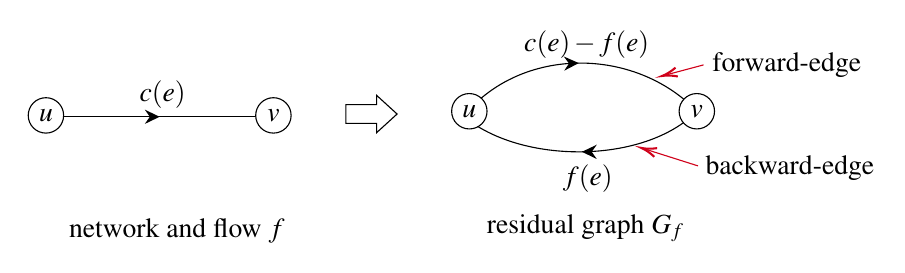
\begin{tikzpicture}[x=0.5pt,y=0.5pt,yscale=-1,xscale=1]
%uncomment if require: \path (0,177); %set diagram left start at 0, and has height of 177

%Curve Lines [id:da27260410535946566] 
\draw    (321,73) .. controls (363,22) and (445,23) .. (489.62,69.5) ;
\draw [shift={(404.33,34.69)}, rotate = 538.0899999999999] [fill={rgb, 255:red, 0; green, 0; blue, 0 }  ][line width=0.08]  [draw opacity=0] (10.72,-5.15) -- (0,0) -- (10.72,5.15) -- (7.12,0) -- cycle    ;
%Curve Lines [id:da29997342467331434] 
\draw    (321,73) .. controls (362,108) and (452,108) .. (489.62,69.5) ;
\draw [shift={(406.58,98.81)}, rotate = 0.2] [fill={rgb, 255:red, 0; green, 0; blue, 0 }  ][line width=0.08]  [draw opacity=0] (10.72,-5.15) -- (0,0) -- (10.72,5.15) -- (7.12,0) -- cycle    ;
%Straight Lines [id:da010972519675235493] 
\draw    (183.62,73.5) -- (19.22,73.5) ;
\draw [shift={(101.42,73.5)}, rotate = 180] [fill={rgb, 255:red, 0; green, 0; blue, 0 }  ][line width=0.08]  [draw opacity=0] (10.72,-5.15) -- (0,0) -- (10.72,5.15) -- (7.12,0) -- cycle    ;
%Shape: Ellipse [id:dp48830544834331435] 
\draw  [fill={rgb, 255:red, 255; green, 255; blue, 255 }  ,fill opacity=1 ] (6.43,72.5) .. controls (6.43,65.44) and (12.15,59.71) .. (19.22,59.71) .. controls (26.28,59.71) and (32.01,65.44) .. (32.01,72.5) .. controls (32.01,79.57) and (26.28,85.29) .. (19.22,85.29) .. controls (12.15,85.29) and (6.43,79.57) .. (6.43,72.5) -- cycle ;
%Shape: Ellipse [id:dp5269749982517756] 
\draw  [fill={rgb, 255:red, 255; green, 255; blue, 255 }  ,fill opacity=1 ] (170.83,72.5) .. controls (170.83,65.44) and (176.56,59.71) .. (183.62,59.71) .. controls (190.69,59.71) and (196.41,65.44) .. (196.41,72.5) .. controls (196.41,79.57) and (190.69,85.29) .. (183.62,85.29) .. controls (176.56,85.29) and (170.83,79.57) .. (170.83,72.5) -- cycle ;
%Shape: Ellipse [id:dp19207664116491352] 
\draw  [fill={rgb, 255:red, 255; green, 255; blue, 255 }  ,fill opacity=1 ] (312.43,69.5) .. controls (312.43,62.44) and (318.15,56.71) .. (325.22,56.71) .. controls (332.28,56.71) and (338.01,62.44) .. (338.01,69.5) .. controls (338.01,76.57) and (332.28,82.29) .. (325.22,82.29) .. controls (318.15,82.29) and (312.43,76.57) .. (312.43,69.5) -- cycle ;
%Shape: Ellipse [id:dp6327110520101094] 
\draw  [fill={rgb, 255:red, 255; green, 255; blue, 255 }  ,fill opacity=1 ] (476.83,69.5) .. controls (476.83,62.44) and (482.56,56.71) .. (489.62,56.71) .. controls (496.69,56.71) and (502.41,62.44) .. (502.41,69.5) .. controls (502.41,76.57) and (496.69,82.29) .. (489.62,82.29) .. controls (482.56,82.29) and (476.83,76.57) .. (476.83,69.5) -- cycle ;
%Right Arrow [id:dp9435587998338902] 
\draw   (236,64.75) -- (258.2,64.75) -- (258.2,58) -- (273,71.5) -- (258.2,85) -- (258.2,78.25) -- (236,78.25) -- cycle ;
%Straight Lines [id:da786288103209363] 
\draw [color={rgb, 255:red, 208; green, 2; blue, 27 }  ,draw opacity=1 ]   (494.5,36) -- (466.43,43.48) ;
\draw [shift={(464.5,44)}, rotate = 345.07] [color={rgb, 255:red, 208; green, 2; blue, 27 }  ,draw opacity=1 ][line width=0.75]    (10.93,-3.29) .. controls (6.95,-1.4) and (3.31,-0.3) .. (0,0) .. controls (3.31,0.3) and (6.95,1.4) .. (10.93,3.29)   ;
%Straight Lines [id:da5256035535625604] 
\draw [color={rgb, 255:red, 208; green, 2; blue, 27 }  ,draw opacity=1 ]   (490.5,109) -- (451.41,96.6) ;
\draw [shift={(449.5,96)}, rotate = 377.59000000000003] [color={rgb, 255:red, 208; green, 2; blue, 27 }  ,draw opacity=1 ][line width=0.75]    (10.93,-3.29) .. controls (6.95,-1.4) and (3.31,-0.3) .. (0,0) .. controls (3.31,0.3) and (6.95,1.4) .. (10.93,3.29)   ;

% Text Node
\draw (183.62,72.5) node   [align=left] {$\displaystyle v$};
% Text Node
\draw (19.22,72.5) node   [align=left] {$\displaystyle u$};
% Text Node
\draw (85,45.5) node [anchor=north west][inner sep=0.75pt]   [align=left] {$\displaystyle c( e)$};
% Text Node
\draw (489.62,69.5) node   [align=left] {$\displaystyle v$};
% Text Node
\draw (325.22,69.5) node   [align=left] {$\displaystyle u$};
% Text Node
\draw (363,9.5) node [anchor=north west][inner sep=0.75pt]   [align=left] {$\displaystyle c( e) -f( e)$};
% Text Node
\draw (391,106.5) node [anchor=north west][inner sep=0.75pt]   [align=left] {$\displaystyle f( e)$};
% Text Node
\draw (34,145) node [anchor=north west][inner sep=0.75pt]   [align=left] {network and flow $\displaystyle f$};
% Text Node
\draw (336,142) node [anchor=north west][inner sep=0.75pt]   [align=left] {residual graph $\displaystyle G_{f}$};
% Text Node
\draw (499,25) node [anchor=north west][inner sep=0.75pt]   [align=left] {forward-edge};
% Text Node
\draw (494,100) node [anchor=north west][inner sep=0.75pt]   [align=left] {backward-edge};


\end{tikzpicture}

}
\caption{Constructing the minimum vertex cover using the residual graph w.r.t.\ the maximum flow.}
\label{fig:residual}
\end{figure}

We first show that $V_1$ is a vertex cover of the bipartite graph. This is equivalent to show
the following fact.  Can you spot it in Figure~\ref{fig:residual}?
\begin{fact} \label{noedges}
In the bipartite graph, there does not exist any edge between $(X\cap S^*)$ and $(Y\cap T^*)$. 
\end{fact}
\emph{Proof.} Suppose conversely that there exists an edge $(u,v)\in E$ with $u\in X\cap S^*$ and $v\in Y\cap T^*$.
Consider $f^*(u,v)$, i.e., the amount of flow carried by this edge in the maximum flow $f^*$.
There are two possibilities~(as all capacities are 1): either $f^*(u,v) = 0$ or $f^*(u,v) = 1$. See Figure~\ref{fig:proof}.
\vspace*{-\topsep}
\begin{enumerate}
\item Suppose that $f^*(u,v) = 0$. Then in the residual graph $G'_{f^*}$ this edge becomes a forward edge $(u,v)$.
Then $v$ must be in $S^*$ as $s$ can reach $u$ and $u$ can reach $v$ following this edge, a contradiction
to the assumption that $v\in T^*$.
\item Suppose that $f^*(u,v) = 1$. Then we must have that $f^*(s,u) = f^*(v,t) = 1$, in order to make $u$ and $v$ satisfy
the conservation condition. Therefore, in the residual graph $G'_{f^*}$, all these three edges become backward edges.
Think: in the residual graph why $u$ is reachable from $s$?
Clearly $u$ cannot be reached from $s$ using edge $(s,u)$ as it's edge $(u,s)$ that appears in the residual graph.
Hence, there must exist a path from $s$ to $u$ using other intermediate vertices.
Assume that on this path the vertex before $u$ is $w$, i.e., edge $(w,u)$ appears in the residual graph.
Notice that $w$ cannot be $v$, as otherwise this implies that $s$ can reach $v$ which contradicts to that $v\in T^*$.
Since edge $(w,u)$ is also a backward-edge, we have that $f^*(u,w) = 1$.
Combined, we have a contradiction, as it's not possible to have both $f^*(u,v) = 1$ and $f^*(u,w) = 1$
because this breaks the capacity condition of edge $(s,u)$. \qed
\end{enumerate}

\begin{figure}[t]
\centering{

\tikzset{every picture/.style={line width=0.75pt}} %set default line width to 0.75pt        

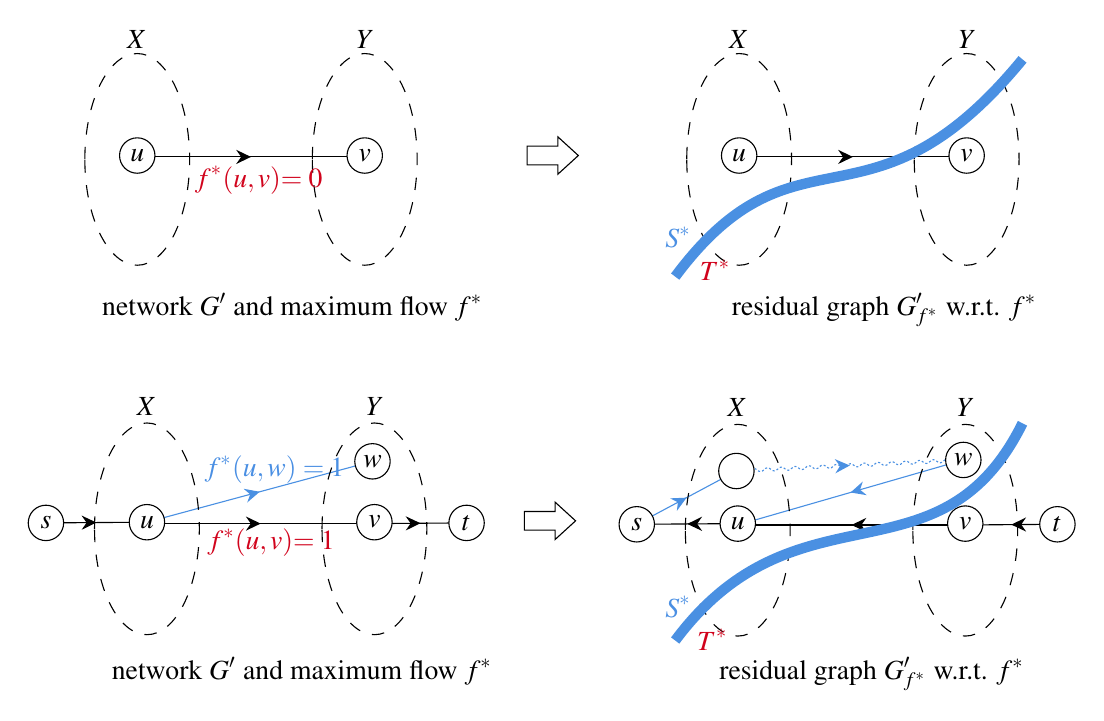
\begin{tikzpicture}[x=0.5pt,y=0.5pt,yscale=-1,xscale=1]
%uncomment if require: \path (0,489); %set diagram left start at 0, and has height of 489

%Straight Lines [id:da6191213399358775] 
\draw [color={rgb, 255:red, 74; green, 144; blue, 226 }  ,draw opacity=1 ]   (256.22,322.5) -- (93.22,366.5) ;
\draw [shift={(174.72,344.5)}, rotate = 164.89] [fill={rgb, 255:red, 74; green, 144; blue, 226 }  ,fill opacity=1 ][line width=0.08]  [draw opacity=0] (10.72,-5.15) -- (0,0) -- (10.72,5.15) -- (7.12,0) -- cycle    ;
%Straight Lines [id:da8327265709083349] 
\draw [color={rgb, 255:red, 74; green, 144; blue, 226 }  ,draw opacity=1 ]   (447.22,368) -- (519.22,329.5) ;
\draw [shift={(483.22,348.75)}, rotate = 511.87] [fill={rgb, 255:red, 74; green, 144; blue, 226 }  ,fill opacity=1 ][line width=0.08]  [draw opacity=0] (10.72,-5.15) -- (0,0) -- (10.72,5.15) -- (7.12,0) -- cycle    ;
%Straight Lines [id:da8516915581936988] 
\draw [color={rgb, 255:red, 74; green, 144; blue, 226 }  ,draw opacity=1 ] [dash pattern={on 0.75pt off 0.75pt}]  (519.22,329.5) .. controls (520.8,327.76) and (522.46,327.68) .. (524.21,329.26) .. controls (525.96,330.85) and (527.62,330.77) .. (529.21,329.02) .. controls (530.79,327.27) and (532.45,327.19) .. (534.2,328.77) .. controls (535.95,330.36) and (537.61,330.28) .. (539.19,328.53) .. controls (540.78,326.78) and (542.44,326.7) .. (544.19,328.29) .. controls (545.94,329.87) and (547.6,329.79) .. (549.18,328.04) .. controls (550.77,326.29) and (552.43,326.21) .. (554.18,327.8) .. controls (555.93,329.39) and (557.59,329.31) .. (559.17,327.56) .. controls (560.76,325.81) and (562.42,325.73) .. (564.17,327.31) .. controls (565.92,328.9) and (567.58,328.82) .. (569.16,327.07) .. controls (570.74,325.32) and (572.4,325.24) .. (574.15,326.83) .. controls (575.9,328.41) and (577.56,328.33) .. (579.15,326.58) .. controls (580.73,324.83) and (582.39,324.75) .. (584.14,326.34) .. controls (585.89,327.92) and (587.55,327.84) .. (589.14,326.09) .. controls (590.72,324.34) and (592.38,324.26) .. (594.13,325.85) .. controls (595.88,327.44) and (597.54,327.36) .. (599.12,325.61) .. controls (600.71,323.86) and (602.37,323.78) .. (604.12,325.36) .. controls (605.87,326.95) and (607.53,326.87) .. (609.11,325.12) .. controls (610.7,323.37) and (612.36,323.29) .. (614.11,324.88) .. controls (615.86,326.46) and (617.52,326.38) .. (619.1,324.63) .. controls (620.68,322.88) and (622.34,322.8) .. (624.09,324.39) .. controls (625.84,325.98) and (627.5,325.9) .. (629.09,324.15) .. controls (630.67,322.4) and (632.33,322.32) .. (634.08,323.9) .. controls (635.83,325.49) and (637.49,325.41) .. (639.08,323.66) .. controls (640.66,321.91) and (642.32,321.83) .. (644.07,323.41) .. controls (645.82,325) and (647.48,324.92) .. (649.06,323.17) .. controls (650.65,321.42) and (652.31,321.34) .. (654.06,322.93) .. controls (655.81,324.51) and (657.47,324.43) .. (659.05,322.68) .. controls (660.64,320.93) and (662.3,320.85) .. (664.05,322.44) .. controls (665.8,324.03) and (667.46,323.95) .. (669.04,322.2) .. controls (670.62,320.45) and (672.28,320.37) .. (674.03,321.95) .. controls (675.78,323.54) and (677.44,323.46) .. (679.03,321.71) -- (683.22,321.5) -- (683.22,321.5) ;
\draw [shift={(601.22,325.5)}, rotate = 537.21] [fill={rgb, 255:red, 74; green, 144; blue, 226 }  ,fill opacity=1 ][line width=0.08]  [draw opacity=0] (10.72,-5.15) -- (0,0) -- (10.72,5.15) -- (7.12,0) -- cycle    ;
%Straight Lines [id:da8322109543199766] 
\draw [color={rgb, 255:red, 74; green, 144; blue, 226 }  ,draw opacity=1 ]   (683.22,321.5) -- (520.22,368.5) ;
\draw [shift={(601.72,345)}, rotate = 343.91999999999996] [fill={rgb, 255:red, 74; green, 144; blue, 226 }  ,fill opacity=1 ][line width=0.08]  [draw opacity=0] (10.72,-5.15) -- (0,0) -- (10.72,5.15) -- (7.12,0) -- cycle    ;
%Straight Lines [id:da577325970602598] 
\draw    (250.62,102.5) -- (86.22,102.5) ;
\draw [shift={(168.42,102.5)}, rotate = 180] [fill={rgb, 255:red, 0; green, 0; blue, 0 }  ][line width=0.08]  [draw opacity=0] (10.72,-5.15) -- (0,0) -- (10.72,5.15) -- (7.12,0) -- cycle    ;
%Shape: Ellipse [id:dp513666224672568] 
\draw  [fill={rgb, 255:red, 255; green, 255; blue, 255 }  ,fill opacity=1 ] (73.43,101.5) .. controls (73.43,94.44) and (79.15,88.71) .. (86.22,88.71) .. controls (93.28,88.71) and (99.01,94.44) .. (99.01,101.5) .. controls (99.01,108.57) and (93.28,114.29) .. (86.22,114.29) .. controls (79.15,114.29) and (73.43,108.57) .. (73.43,101.5) -- cycle ;
%Shape: Ellipse [id:dp9236001904458527] 
\draw  [fill={rgb, 255:red, 255; green, 255; blue, 255 }  ,fill opacity=1 ] (237.83,101.5) .. controls (237.83,94.44) and (243.56,88.71) .. (250.62,88.71) .. controls (257.69,88.71) and (263.41,94.44) .. (263.41,101.5) .. controls (263.41,108.57) and (257.69,114.29) .. (250.62,114.29) .. controls (243.56,114.29) and (237.83,108.57) .. (237.83,101.5) -- cycle ;
%Right Arrow [id:dp2218646176992478] 
\draw   (368,94.75) -- (390.2,94.75) -- (390.2,88) -- (405,101.5) -- (390.2,115) -- (390.2,108.25) -- (368,108.25) -- cycle ;
%Shape: Ellipse [id:dp7576706437482376] 
\draw  [dash pattern={on 4.5pt off 4.5pt}] (48.34,104.29) .. controls (48.34,62.04) and (65.3,27.79) .. (86.22,27.79) .. controls (107.14,27.79) and (124.09,62.04) .. (124.09,104.29) .. controls (124.09,146.54) and (107.14,180.79) .. (86.22,180.79) .. controls (65.3,180.79) and (48.34,146.54) .. (48.34,104.29) -- cycle ;
%Shape: Ellipse [id:dp019919118199761776] 
\draw  [dash pattern={on 4.5pt off 4.5pt}] (212.75,104.29) .. controls (212.75,62.04) and (229.7,27.79) .. (250.62,27.79) .. controls (271.54,27.79) and (288.5,62.04) .. (288.5,104.29) .. controls (288.5,146.54) and (271.54,180.79) .. (250.62,180.79) .. controls (229.7,180.79) and (212.75,146.54) .. (212.75,104.29) -- cycle ;
%Straight Lines [id:da8311742548484229] 
\draw    (685.62,102.5) -- (521.22,102.5) ;
\draw [shift={(603.42,102.5)}, rotate = 180] [fill={rgb, 255:red, 0; green, 0; blue, 0 }  ][line width=0.08]  [draw opacity=0] (10.72,-5.15) -- (0,0) -- (10.72,5.15) -- (7.12,0) -- cycle    ;
%Shape: Ellipse [id:dp9405415347638398] 
\draw  [fill={rgb, 255:red, 255; green, 255; blue, 255 }  ,fill opacity=1 ] (508.43,101.5) .. controls (508.43,94.44) and (514.15,88.71) .. (521.22,88.71) .. controls (528.28,88.71) and (534.01,94.44) .. (534.01,101.5) .. controls (534.01,108.57) and (528.28,114.29) .. (521.22,114.29) .. controls (514.15,114.29) and (508.43,108.57) .. (508.43,101.5) -- cycle ;
%Shape: Ellipse [id:dp11646647893691375] 
\draw  [fill={rgb, 255:red, 255; green, 255; blue, 255 }  ,fill opacity=1 ] (672.83,101.5) .. controls (672.83,94.44) and (678.56,88.71) .. (685.62,88.71) .. controls (692.69,88.71) and (698.41,94.44) .. (698.41,101.5) .. controls (698.41,108.57) and (692.69,114.29) .. (685.62,114.29) .. controls (678.56,114.29) and (672.83,108.57) .. (672.83,101.5) -- cycle ;
%Shape: Ellipse [id:dp9449855279419199] 
\draw  [dash pattern={on 4.5pt off 4.5pt}] (483.34,104.29) .. controls (483.34,62.04) and (500.3,27.79) .. (521.22,27.79) .. controls (542.14,27.79) and (559.09,62.04) .. (559.09,104.29) .. controls (559.09,146.54) and (542.14,180.79) .. (521.22,180.79) .. controls (500.3,180.79) and (483.34,146.54) .. (483.34,104.29) -- cycle ;
%Shape: Ellipse [id:dp97494012923029] 
\draw  [dash pattern={on 4.5pt off 4.5pt}] (647.75,104.29) .. controls (647.75,62.04) and (664.7,27.79) .. (685.62,27.79) .. controls (706.54,27.79) and (723.5,62.04) .. (723.5,104.29) .. controls (723.5,146.54) and (706.54,180.79) .. (685.62,180.79) .. controls (664.7,180.79) and (647.75,146.54) .. (647.75,104.29) -- cycle ;
%Straight Lines [id:da25721893854693145] 
\draw    (93.22,366.5) -- (20.22,367) ;
\draw [shift={(56.72,366.75)}, rotate = 179.61] [fill={rgb, 255:red, 0; green, 0; blue, 0 }  ][line width=0.08]  [draw opacity=0] (10.72,-5.15) -- (0,0) -- (10.72,5.15) -- (7.12,0) -- cycle    ;
%Straight Lines [id:da4797079273399141] 
\draw    (324.22,367) -- (257.62,367.5) ;
\draw [shift={(290.92,367.25)}, rotate = 179.57] [fill={rgb, 255:red, 0; green, 0; blue, 0 }  ][line width=0.08]  [draw opacity=0] (10.72,-5.15) -- (0,0) -- (10.72,5.15) -- (7.12,0) -- cycle    ;
%Straight Lines [id:da0639605968996434] 
\draw    (257.62,367.5) -- (93.22,367.5) ;
\draw [shift={(175.42,367.5)}, rotate = 180] [fill={rgb, 255:red, 0; green, 0; blue, 0 }  ][line width=0.08]  [draw opacity=0] (10.72,-5.15) -- (0,0) -- (10.72,5.15) -- (7.12,0) -- cycle    ;
%Shape: Ellipse [id:dp7215149302709682] 
\draw  [fill={rgb, 255:red, 255; green, 255; blue, 255 }  ,fill opacity=1 ] (80.43,366.5) .. controls (80.43,359.44) and (86.15,353.71) .. (93.22,353.71) .. controls (100.28,353.71) and (106.01,359.44) .. (106.01,366.5) .. controls (106.01,373.57) and (100.28,379.29) .. (93.22,379.29) .. controls (86.15,379.29) and (80.43,373.57) .. (80.43,366.5) -- cycle ;
%Shape: Ellipse [id:dp10876362413389085] 
\draw  [fill={rgb, 255:red, 255; green, 255; blue, 255 }  ,fill opacity=1 ] (244.83,366.5) .. controls (244.83,359.44) and (250.56,353.71) .. (257.62,353.71) .. controls (264.69,353.71) and (270.41,359.44) .. (270.41,366.5) .. controls (270.41,373.57) and (264.69,379.29) .. (257.62,379.29) .. controls (250.56,379.29) and (244.83,373.57) .. (244.83,366.5) -- cycle ;
%Shape: Ellipse [id:dp34296507659419695] 
\draw  [dash pattern={on 4.5pt off 4.5pt}] (55.34,371.29) .. controls (55.34,329.04) and (72.3,294.79) .. (93.22,294.79) .. controls (114.14,294.79) and (131.09,329.04) .. (131.09,371.29) .. controls (131.09,413.54) and (114.14,447.79) .. (93.22,447.79) .. controls (72.3,447.79) and (55.34,413.54) .. (55.34,371.29) -- cycle ;
%Shape: Ellipse [id:dp8298689489920419] 
\draw  [dash pattern={on 4.5pt off 4.5pt}] (219.75,371.29) .. controls (219.75,329.04) and (236.7,294.79) .. (257.62,294.79) .. controls (278.54,294.79) and (295.5,329.04) .. (295.5,371.29) .. controls (295.5,413.54) and (278.54,447.79) .. (257.62,447.79) .. controls (236.7,447.79) and (219.75,413.54) .. (219.75,371.29) -- cycle ;
%Shape: Ellipse [id:dp9137920481521634] 
\draw  [fill={rgb, 255:red, 255; green, 255; blue, 255 }  ,fill opacity=1 ] (7.43,367) .. controls (7.43,359.94) and (13.15,354.21) .. (20.22,354.21) .. controls (27.28,354.21) and (33.01,359.94) .. (33.01,367) .. controls (33.01,374.07) and (27.28,379.79) .. (20.22,379.79) .. controls (13.15,379.79) and (7.43,374.07) .. (7.43,367) -- cycle ;
%Shape: Ellipse [id:dp215960632133124] 
\draw  [fill={rgb, 255:red, 255; green, 255; blue, 255 }  ,fill opacity=1 ] (311.43,367) .. controls (311.43,359.94) and (317.15,354.21) .. (324.22,354.21) .. controls (331.28,354.21) and (337.01,359.94) .. (337.01,367) .. controls (337.01,374.07) and (331.28,379.79) .. (324.22,379.79) .. controls (317.15,379.79) and (311.43,374.07) .. (311.43,367) -- cycle ;
%Curve Lines [id:da39738584929269916] 
\draw [color={rgb, 255:red, 74; green, 144; blue, 226 }  ,draw opacity=1 ][line width=3.75]    (475,189) .. controls (563,71) and (615,167) .. (726,32) ;
%Straight Lines [id:da7379384720847889] 
\draw    (520.22,367.5) -- (447.22,368) ;
\draw [shift={(483.72,367.75)}, rotate = 359.61] [fill={rgb, 255:red, 0; green, 0; blue, 0 }  ][line width=0.08]  [draw opacity=0] (10.72,-5.15) -- (0,0) -- (10.72,5.15) -- (7.12,0) -- cycle    ;
%Straight Lines [id:da3670804661459104] 
\draw    (751.22,368) -- (684.62,368.5) ;
\draw [shift={(717.92,368.25)}, rotate = 359.57] [fill={rgb, 255:red, 0; green, 0; blue, 0 }  ][line width=0.08]  [draw opacity=0] (10.72,-5.15) -- (0,0) -- (10.72,5.15) -- (7.12,0) -- cycle    ;
%Straight Lines [id:da21692742405585586] 
\draw    (684.62,368.5) -- (520.22,368.5) ;
\draw [shift={(602.42,368.5)}, rotate = 360] [fill={rgb, 255:red, 0; green, 0; blue, 0 }  ][line width=0.08]  [draw opacity=0] (10.72,-5.15) -- (0,0) -- (10.72,5.15) -- (7.12,0) -- cycle    ;
%Shape: Ellipse [id:dp4921121681649563] 
\draw  [fill={rgb, 255:red, 255; green, 255; blue, 255 }  ,fill opacity=1 ] (507.43,367.5) .. controls (507.43,360.44) and (513.15,354.71) .. (520.22,354.71) .. controls (527.28,354.71) and (533.01,360.44) .. (533.01,367.5) .. controls (533.01,374.57) and (527.28,380.29) .. (520.22,380.29) .. controls (513.15,380.29) and (507.43,374.57) .. (507.43,367.5) -- cycle ;
%Shape: Ellipse [id:dp4020136360807661] 
\draw  [fill={rgb, 255:red, 255; green, 255; blue, 255 }  ,fill opacity=1 ] (671.83,367.5) .. controls (671.83,360.44) and (677.56,354.71) .. (684.62,354.71) .. controls (691.69,354.71) and (697.41,360.44) .. (697.41,367.5) .. controls (697.41,374.57) and (691.69,380.29) .. (684.62,380.29) .. controls (677.56,380.29) and (671.83,374.57) .. (671.83,367.5) -- cycle ;
%Shape: Ellipse [id:dp2784381633198203] 
\draw  [dash pattern={on 4.5pt off 4.5pt}] (482.34,372.29) .. controls (482.34,330.04) and (499.3,295.79) .. (520.22,295.79) .. controls (541.14,295.79) and (558.09,330.04) .. (558.09,372.29) .. controls (558.09,414.54) and (541.14,448.79) .. (520.22,448.79) .. controls (499.3,448.79) and (482.34,414.54) .. (482.34,372.29) -- cycle ;
%Shape: Ellipse [id:dp6984861741222058] 
\draw  [dash pattern={on 4.5pt off 4.5pt}] (646.75,372.29) .. controls (646.75,330.04) and (663.7,295.79) .. (684.62,295.79) .. controls (705.54,295.79) and (722.5,330.04) .. (722.5,372.29) .. controls (722.5,414.54) and (705.54,448.79) .. (684.62,448.79) .. controls (663.7,448.79) and (646.75,414.54) .. (646.75,372.29) -- cycle ;
%Shape: Ellipse [id:dp6691205194220659] 
\draw  [fill={rgb, 255:red, 255; green, 255; blue, 255 }  ,fill opacity=1 ] (434.43,368) .. controls (434.43,360.94) and (440.15,355.21) .. (447.22,355.21) .. controls (454.28,355.21) and (460.01,360.94) .. (460.01,368) .. controls (460.01,375.07) and (454.28,380.79) .. (447.22,380.79) .. controls (440.15,380.79) and (434.43,375.07) .. (434.43,368) -- cycle ;
%Shape: Ellipse [id:dp11182746749852701] 
\draw  [fill={rgb, 255:red, 255; green, 255; blue, 255 }  ,fill opacity=1 ] (738.43,368) .. controls (738.43,360.94) and (744.15,355.21) .. (751.22,355.21) .. controls (758.28,355.21) and (764.01,360.94) .. (764.01,368) .. controls (764.01,375.07) and (758.28,380.79) .. (751.22,380.79) .. controls (744.15,380.79) and (738.43,375.07) .. (738.43,368) -- cycle ;
%Curve Lines [id:da0028084380062078917] 
\draw [color={rgb, 255:red, 74; green, 144; blue, 226 }  ,draw opacity=1 ][line width=3.75]    (475,452) .. controls (563,334) and (666,416) .. (726,295) ;
%Shape: Ellipse [id:dp6641341242010522] 
\draw  [fill={rgb, 255:red, 255; green, 255; blue, 255 }  ,fill opacity=1 ] (506.43,329.5) .. controls (506.43,322.44) and (512.15,316.71) .. (519.22,316.71) .. controls (526.28,316.71) and (532.01,322.44) .. (532.01,329.5) .. controls (532.01,336.57) and (526.28,342.29) .. (519.22,342.29) .. controls (512.15,342.29) and (506.43,336.57) .. (506.43,329.5) -- cycle ;
%Shape: Ellipse [id:dp6412575212172368] 
\draw  [fill={rgb, 255:red, 255; green, 255; blue, 255 }  ,fill opacity=1 ] (670.43,321.5) .. controls (670.43,314.44) and (676.15,308.71) .. (683.22,308.71) .. controls (690.28,308.71) and (696.01,314.44) .. (696.01,321.5) .. controls (696.01,328.57) and (690.28,334.29) .. (683.22,334.29) .. controls (676.15,334.29) and (670.43,328.57) .. (670.43,321.5) -- cycle ;
%Shape: Ellipse [id:dp4382651677301832] 
\draw  [fill={rgb, 255:red, 255; green, 255; blue, 255 }  ,fill opacity=1 ] (243.43,322.5) .. controls (243.43,315.44) and (249.15,309.71) .. (256.22,309.71) .. controls (263.28,309.71) and (269.01,315.44) .. (269.01,322.5) .. controls (269.01,329.57) and (263.28,335.29) .. (256.22,335.29) .. controls (249.15,335.29) and (243.43,329.57) .. (243.43,322.5) -- cycle ;
%Right Arrow [id:dp9788576014249767] 
\draw   (366,358.75) -- (388.2,358.75) -- (388.2,352) -- (403,365.5) -- (388.2,379) -- (388.2,372.25) -- (366,372.25) -- cycle ;

% Text Node
\draw (250.62,101.5) node   [align=left] {$\displaystyle v$};
% Text Node
\draw (86.22,101.5) node   [align=left] {$\displaystyle u$};
% Text Node
\draw (59,199) node [anchor=north west][inner sep=0.75pt]   [align=left] {network $\displaystyle G'$ and maximum flow $\displaystyle f^{*}$};
% Text Node
\draw (77,9.5) node [anchor=north west][inner sep=0.75pt]   [align=left] {$\displaystyle X$};
% Text Node
\draw (243,9.5) node [anchor=north west][inner sep=0.75pt]   [align=left] {$\displaystyle Y$};
% Text Node
\draw (126.09,107.29) node [anchor=north west][inner sep=0.75pt]   [align=left] {$\displaystyle \textcolor[rgb]{0.82,0.01,0.11}{f}\textcolor[rgb]{0.82,0.01,0.11}{^{*}}\textcolor[rgb]{0.82,0.01,0.11}{( u,v}\textcolor[rgb]{0.82,0.01,0.11}{)}\textcolor[rgb]{0.82,0.01,0.11}{=0}$};
% Text Node
\draw (685.62,101.5) node   [align=left] {$\displaystyle v$};
% Text Node
\draw (521.22,101.5) node   [align=left] {$\displaystyle u$};
% Text Node
\draw (514,199) node [anchor=north west][inner sep=0.75pt]   [align=left] {residual graph $\displaystyle G'_{f^{*}}$ w.r.t. $\displaystyle f^{*}$};
% Text Node
\draw (512,9.5) node [anchor=north west][inner sep=0.75pt]   [align=left] {$\displaystyle X$};
% Text Node
\draw (678,9.5) node [anchor=north west][inner sep=0.75pt]   [align=left] {$\displaystyle Y$};
% Text Node
\draw (257.62,366.5) node   [align=left] {$\displaystyle v$};
% Text Node
\draw (93.22,366.5) node   [align=left] {$\displaystyle u$};
% Text Node
\draw (66,462) node [anchor=north west][inner sep=0.75pt]   [align=left] {network $\displaystyle G'$ and maximum flow $\displaystyle f^{*}$};
% Text Node
\draw (84,274.5) node [anchor=north west][inner sep=0.75pt]   [align=left] {$\displaystyle X$};
% Text Node
\draw (250,274.5) node [anchor=north west][inner sep=0.75pt]   [align=left] {$\displaystyle Y$};
% Text Node
\draw (135,369.5) node [anchor=north west][inner sep=0.75pt]   [align=left] {$\displaystyle \textcolor[rgb]{0.82,0.01,0.11}{f}\textcolor[rgb]{0.82,0.01,0.11}{^{*}}\textcolor[rgb]{0.82,0.01,0.11}{( u,v}\textcolor[rgb]{0.82,0.01,0.11}{)}\textcolor[rgb]{0.82,0.01,0.11}{=1}$};
% Text Node
\draw (20.22,367) node   [align=left] {$\displaystyle s$};
% Text Node
\draw (324.22,367) node   [align=left] {$\displaystyle t$};
% Text Node
\draw (466,151) node [anchor=north west][inner sep=0.75pt]   [align=left] {$\displaystyle \textcolor[rgb]{0.29,0.56,0.89}{S}\textcolor[rgb]{0.29,0.56,0.89}{^{*}}$};
% Text Node
\draw (491,175) node [anchor=north west][inner sep=0.75pt]   [align=left] {$\displaystyle \textcolor[rgb]{0.82,0.01,0.11}{T}\textcolor[rgb]{0.82,0.01,0.11}{^{*}}$};
% Text Node
\draw (684.62,367.5) node   [align=left] {$\displaystyle v$};
% Text Node
\draw (520.22,367.5) node   [align=left] {$\displaystyle u$};
% Text Node
\draw (511,275.5) node [anchor=north west][inner sep=0.75pt]   [align=left] {$\displaystyle X$};
% Text Node
\draw (677,275.5) node [anchor=north west][inner sep=0.75pt]   [align=left] {$\displaystyle Y$};
% Text Node
\draw (447.22,368) node   [align=left] {$\displaystyle s$};
% Text Node
\draw (751.22,368) node   [align=left] {$\displaystyle t$};
% Text Node
\draw (466,418) node [anchor=north west][inner sep=0.75pt]   [align=left] {$\displaystyle \textcolor[rgb]{0.29,0.56,0.89}{S}\textcolor[rgb]{0.29,0.56,0.89}{^{*}}$};
% Text Node
\draw (489,442) node [anchor=north west][inner sep=0.75pt]   [align=left] {$\displaystyle \textcolor[rgb]{0.82,0.01,0.11}{T}\textcolor[rgb]{0.82,0.01,0.11}{^{*}}$};
% Text Node
\draw (683.22,321.5) node   [align=left] {$\displaystyle w$};
% Text Node
\draw (256.22,322.5) node   [align=left] {$\displaystyle w$};
% Text Node
\draw (133,316.5) node [anchor=north west][inner sep=0.75pt]   [align=left] {$\displaystyle \textcolor[rgb]{0.29,0.56,0.89}{f^{*}( u,w) =1}$};
% Text Node
\draw (505,462) node [anchor=north west][inner sep=0.75pt]   [align=left] {residual graph $\displaystyle G'_{f^{*}}$ w.r.t. $\displaystyle f^{*}$};


\end{tikzpicture}

}
\caption{Illustrating the two cases in proving Fact~\ref{noedges}.}
\label{fig:proof}
\end{figure}

Above fact immediately gives that $V_1$ is a vertex cover of the bipartite graph.
See Figure~\ref{fig:residual} for a sketch of $G'$.
We now show that $V_1$ is also a minimum vertex cover.
Consider the capacity of $s$-$t$ cut $(S^*, T^*)$. 
Since there is no edge between $X\cap S^*$ and $Y\cap T^*$, we have
that $c(S^*, T^*) = |X\cap T^*| + |Y\cap S^*|$, as every edge has a capacity of 1.
According to the max-flow min-cut theorem, we know 
$c(S^*, T^*) = |f^*|$. We also proved that $|M| = |f^*|$. Combined, 
we have $|V_1| = |X\cap T^*| + |Y\cap S^*| = c(S^*, T^*) = |f^*| = |M|$, as desired.

We summarize the maximum matching problem and the minimum vertex cover problem below.
\vspace*{-\topsep}
\begin{enumerate}
\item For any \emph{bipartite graph}, its maximum matching
and minimum vertex cover always have equal cardinality,
and such maximum matching and minimum vertex cover
can be found using above algorithm which runs in polynomial-time.
\item For \emph{general} undirected graphs, the size of
any vertex cover is always an upper bound of that of any matching,
but a gap might exist on graphs with odd-length cycles.
The minimum vertex cover problem (on general undirected graphs) is NP-hard, i.e., there does not
exist polynomial-time (optimal) algorithm for it.
But the maximum matching problem (on general undirected graphs) can be solved in polynomial-time,
for example, with the Blossom algorithm~(Edmonds, 1961).
\end{enumerate}

\end{document}
